\documentclass[12pt]{jarticle}
\usepackage[utf8]{inputenc}
\usepackage[top=30truemm, bottom=30truemm, left=20truemm, right=20truemm]{geometry}
\usepackage{amsmath}
\usepackage{amssymb}
\usepackage{mathtools}
\usepackage{siunitx}
\usepackage{bm}
\usepackage[dvipdfmx]{graphicx}
\usepackage[dvipdfmx]{color}
\usepackage[subrefformat=parens]{subcaption}
\usepackage{booktabs}
\usepackage{tabularx}
\usepackage{tocloft}
\usepackage{enumerate}
\usepackage{url}
\usepackage{multirow}
\usepackage{caption}
\usepackage{enumitem}
\usepackage{makecell}
\usepackage{array}
\usepackage{algorithm}
\usepackage{algpseudocode}

\numberwithin{equation}{section}    % 数式番号にセクション番号をつける
\numberwithin{figure}{section}      % 図番号にセクション
\numberwithin{table}{section}      % 図番号にセクション

% \renewcommand{\figurename}{Fig.}    % 図 -> Fig.
% \renewcommand{\tablename}{Table }   % 表 -> Table

\renewcommand{\baselinestretch}{1.1}
\newcommand{\ie}{\textit{i}.\textit{e}.}

\newlength{\figcaptionskip}
\setlength{\figcaptionskip}{5pt} % 図のキャプション間隔
\newlength{\tabcaptionskip}
\setlength{\tabcaptionskip}{-5pt} % 表のキャプション間隔
\captionsetup[figure]{skip=\figcaptionskip}
\captionsetup[table]{skip=\tabcaptionskip}

\setlist[enumerate]{topsep=5pt, partopsep=5pt, itemsep=0pt, parsep=0pt}
\setlength{\topsep}{5pt}
\setlength{\partopsep}{5pt}


\begin{document}

\begin{titlepage}
    \begin{center}
        {\Large 2024年度後期 修士論文}
        \vspace{120truept}

        {\huge 深層学習による口唇音声変換に関する研究}
        \vspace{30truept}

        {\huge A Study on the Conversion from Lip-Video to Speech Using a Deep Learning Technique}
        \vspace{120truept}

        {\Large 2025年月日}
        \vspace{10truept}

        {\Large 九州大学芸術工学府音響設計コース}
        \vspace{70truept}

        {\Large 2DS23095M}
        \vspace{10truept}

        {\Large 南 汰翼}
        \vspace{10truept}

        {\Large MINAMI Taisuke}
        \vspace{30truept}

        {\Large 研究指導教員 鏑木 時彦 教授}
    \end{center}
\end{titlepage}

\section*{概要}
\thispagestyle{empty}
\clearpage

\setcounter{tocdepth}{2}
\tableofcontents
\thispagestyle{empty}
\clearpage

\pagestyle{plain}
\setcounter{page}{1}

\section{序論}
\subsection{背景}
音声は基本的なコミュニケーション手段として、人々の日常生活において重要な役割を果たしている。しかし、癌などの病気で喉頭を摘出すると、声帯振動による音声生成が不可能になり、従来の発声手段を失う。このような場合の代用音声手法として、電気式人工喉頭や食道発声、シャント発声があるが、自然で聞き取りやすい音声を生成することが難しかったり、習得に訓練を必要としたり、器具の交換のための定期的な手術を必要とするといった課題がある。これに対して本研究では、新たな代用音声手法として、深層学習を活用して口唇の動きと音声波形の関係性を学習することで、口唇の動きから音声を合成するアプローチを提案する。この手法により、訓練や手術を必要とせずとも、自然な声でのコミュニケーションを可能にすることを目指す。

% 音声は基本的なコミュニケーションの手段であり、人と人とのコミュニケーションの場面において、重要な役割を果たしている。音声は、肺からの呼気流による声帯の振動が音源波を生成し、声道特性に伴ったフィルタリングと口唇からの放射特性に従って生成される。これより、音声の生成には音源を作り出す声帯やその制御のための喉頭、舌や口唇といった調音器官の働きが重要となる。しかし、癌などの重い病気で喉頭を摘出した場合、音源波を生成することができなくなるため、これまで通り発声を行うことが不可能になってしまう。このようなコミュニケーション機能の喪失に対し、現在でも電気式人工喉頭や食道発声、シャント発声といった代用音声手法が存在する。電気式人工喉頭では、専用の発振器を顎下に当てて振動を加えることにより、それを音源とした発声を行う。発振器を用意すれば容易に発声することが可能であるが、生成される音声のピッチが発振器の振動に依存してしまうため、抑揚のない単調な音声になってしまう。食道発声では、まず口や鼻から食道内に空気を取り込み、その空気を逆流させることで食道入口部の粘膜を振動させることによって発声する。電気式人工喉頭と違って道具を必要とせず、ピッチも本人が調節できるが、その習得に長期間の訓練を要する。シャント発声では、手術によって気管と食道を繋ぐ管を設ける。これにより、息を吐き出す際に設けられた喉の穴を手で塞ぐことによって肺からの呼気流が食道に流れる。そのため、食道発声と同様に粘膜の振動を音源とし、発声することが可能となる。習得は容易であり、比較的自然に話すことが可能となるが、設けられた管を交換するための定期的な手術が必要となる。このように、現在用いられている代用音声手法にはそれぞれデメリットが存在する。

% これに対し、本研究ではビデオカメラで撮影した口唇の動きから音声合成を行うことによる、新たな代用音声手法を検討する。本来、音声は声帯の振動や声道の形状に依存して生成されるものであり、口唇の動きのみから音声波形を直接推定することは困難である。そこで、近年画像や自然言語処理、音声といった分野において成果を上げている深層学習を活用し、口唇の動きと音声の間の関係を学習することで推定を行う。これにより、従来の代用音声手法よりも自然性の高い音声を、訓練や定期的な手術の必要なく提供することを目指す。

% これまでの動画音声合成は英語が中心に検討が進んでおり、近年ではYouTube上のデータを収集、処理することによって構築した大規模データセット\cite{afouras2018lrs3,chung2018voxceleb2}を用いることで、大規模で表現力の高いモデルが構築可能となっている。特に、従来行われてきた教師あり学習のみならず、動画と音声の関係性を自己教師あり学習(Self Supervised Learning; SSL)によって学習し、そのモデルを動画音声合成や、動画からテキストを推定するVisual Speech Recognition(VSR)にFineTuningするアプローチが提案され、その有効性が示されている。自己教師あり学習モデルにもいくつかの種類があり、近年多くの研究で応用例のあるAVHuBERT\cite{shi2022learning}は、動画・音声の入力領域においてマスクされた区間の予測と、予測対象の更新を繰り返して学習を進めていくモデルである。予測対象の更新は5回行われ、1回目は音声波形から計算されるMFCCをクラスタリングした結果を利用するが、2回目以降はモデルの中間特徴量をクラスタリングした結果を新たな予測対象に設定する。更新のたびに再度モデルをランダム初期化して再学習するが、その予測対象の複雑さが増していくことによって、学習が促進されるようなメカニズムとなっている。また、これに類似したVATLM\cite{zhu2023vatlm}は、動画と音声のみならずテキストも加えた学習によって、精度改善を達成した。その他、StudentとTeacherという二つのネットワークを利用し、Teacherから出力される特徴量をStudentがマスクされた入力から予測することによって学習を進めるRAVEn\cite{haliassos2022jointly}やAV-data2vec\cite{lian2023av}、RAVEnの改善版として提案されたBRAVEn\cite{haliassos2024braven}など、多くのモデルが提案されている。

近年の動画音声合成では、LRS3\cite{afouras2018lrs3}やVoxCeleb2\cite{chung2018voxceleb2}などの大規模データセットを活用して構築された、自己教師あり学習(Self Supervised Learning; SSL)モデルをFineTuningすることの有効性が示されている。特に、近年の動画音声合成においてはAVHuBERT\cite{shi2022learning}というモデルが動画からの特徴抽出器として採用される場合が多い。AVHuBERTは、動画と音声の対応関係をMasked Predictionという自己教師あり学習方法により捉えたモデルであり、Modality Dropoutという工夫により、自己教師あり学習時には動画と音声の両方を入力とするものの、FineTuning時には動画あるいは音声のみを入力とできる柔軟性を持ち合わせている。これに加え、従来の動画音声においては動画からの予測対象としてメルスペクトログラムが選択されることが多かったが、近年ではこれにテキストや、音声SSLモデルであるHuBERTを利用して得られた離散特徴量を合わせて予測対象とする、マルチタスク学習の有効性が示されている\cite{kim2023lip_multitask,choi2023intelligible}。

% 近年の動画音声合成では、こういったSSLモデルを動画からの特徴抽出器として活用しつつ、さらなる工夫によって精度改善を達成している。動画音声合成について、\cite{kim2023lip_multitask}では予測対象として従来用いられてきたメルスペクトログラムに加え、テキストを予測するマルチタスク学習手法を提案した。損失においては上記の二つに加え、予測したメルスペクトログラムを事前学習済みの音声認識モデルに入力して得られる特徴表現も採用した。音声波形はメルスペクトログラムに対してGriffin-Limアルゴリズムを適用することで獲得しており、従来のメルスペクトログラムのみを損失とする手法に対して客観評価指標における改善を達成した。これに続き、\cite{choi2023intelligible}では前述した手法がテキストアノテーションされたデータのみにしか用いることができないという課題を解消するため、テキストと同様に言語的な情報を持つと考えられている、音声SSLモデルのHuBERT\cite{hsu2021hubert}を利用して得られるHuBERT離散特徴量を用いる手法を提案した。ここで、HuBERT離散特徴量は、HuBERTのTransformer層出力に対してk-means法によるクラスタリングを適用することで得られる。また、予測されたメルスペクトログラムとHuBERT離散特徴量の両方を入力とするMulti-input Vocoderと、Multi-input Vocoderの学習時にメルスペクトログラムにノイズをかけるデータ拡張手法を合わせて提案し、客観評価と主観評価の両方で\cite{kim2023lip_multitask}を含む既存手法に対する改善を達成した。加えて、ここではAVHuBERTの転移学習についても合わせて検討が行われ、これによってさらに性能を改善できることを示した。手法\cite{choi2023intelligible}に関連して、上記のようなマルチタスク学習手法以外にも、HuBERT離散特徴量や、離散化する前の連続特徴量を音声波形までの中間特徴量として扱う手法が存在する。例えば、\cite{hsu2023revise}ではメルスペクトログラムの推定を行わず、HuBERT離散特徴量のみを推定して音声波形に変換する手法が提案された。\cite{choi2023intelligible}では離散化におけるクラスタ数を200としていたのに対して、\cite{hsu2023revise}ではクラスタ数を2000と大きく取っている点で実装が異なっている。メルスペクトログラムを省略する分、クラスタリングによる情報圧縮の程度を軽減することで、音声波形への変換に十分な情報を保持する目的があると考えられる。また、\cite{choi2023intelligible}や\cite{hsu2023revise}ではAVHuBERTを直接動画音声合成にFineTuningしていた一方で、\cite{sahipjohn2023robustl2s}ではAVHuBERTをVSRによってFineTuningし、その後重みを固定した上で特徴抽出器として利用するアプローチを提案している。この手法では、VSRでFineTuningされたAVHuBERTから得られる動画特徴量を入力とし、HuBERT特徴量を予測するネットワークが追加で学習され、HuBERT特徴量のみから音声波形に変換するボコーダを用いることで動画音声合成が実現された。ここで、HuBERT特徴量と表した予測対象について、この研究では他の研究においても検討されたHuBERT離散特徴量だけでなく、クラスタリングによって離散化する前の連続値を用いる場合、離散値と連続値の両方を予測対象とする場合が検討され、連続値のみを予測対象とした場合が最も客観評価指標が優れていたことが示されている。検討された離散値のクラスタ数が100であったことと、\cite{hsu2023revise}の検討とを合わせると、HuBERT離散特徴量のみを用いて音声波形に変換するアプローチを取るのであれば、クラスタ数を十分大きく取る必要があることが示唆される。

% 一方VSRについて、\cite{yeo2024akvsr}では、HuBERT離散特徴量から純粋な言語情報のみを持つCompact Audio Memoryを構築し、これを動画特徴量とアテンションで関連付ける手法を提案した。ここで、Compact Audio MemoryはHuBERT離散特徴量、すなわちインデックス系列を学習可能なベクトルに写し、これを入力とした音声認識モデルを学習させることで得られる。この研究では、HuBERT離散特徴量が言語的な情報のみを持った特徴量であると考えつつ、話者性など言語情報以外の情報が含まれる可能性を考慮して、音声認識に最適化された新たなコードブックを構築することで冗長性を排除した。このCompact Audio Memoryは、VSRモデルの学習時にアテンションをとる対象として用いられる。Compact Audio Memoryが言語情報のみを持つ離散的な表現だと考えると、これは予測対象であるテキストとほとんど同一のものとなるから、提案された手法は予測対象と同等な情報に対するアテンションをモデル内部で取ることによって、最終予測値に対する動画からの特徴抽出をうまく行えるようにネットワークを構成したのだと解釈できる。また、\cite{cheng2023opensr}では、AVHuBERTが動画あるいは音声のどちら一方を入力とした場合でも同じ音素空間にマッピングできる点に着目し、VSRのための学習データを少量に絞ったFew-shot Learningや、VSRのための学習データを用いないZero-shot Learningを検討した。特にZero-shot Learningでは、AVHuBERTの重みを固定したまま音声波形を特徴量に変換して音声認識モデルを学習し、その後動画をAVHuBERTに通して特徴量に変換して音声認識モデルへの入力とすることで、VSR用の学習データを用いることなくテキストの推定が可能であることを示した。加えて、\cite{djilali2023lip2vec}では、AVHuBERTを動画特徴抽出器として利用し、音声認識モデルの中間表現を予測するネットワークを学習するアプローチが提案されている。この手法では、AVHuBERTと音声認識モデルの事前学習済み重みを固定した上で、両者の潜在表現間を繋ぐPrior Networkを学習し、動画から得られる特徴量を音声に近い表現に変換する。この変換された表現を音声認識モデルに入力し、テキストを推定することで、VSRを実現している。
% さらに、静止画像と音声から動画を合成するネットワークを構築し、音声認識用のデータセットを用いてVSRの学習データを大量に合成するデータ拡張手法\cite{liu2023synthvsr}や、事前学習済みの音声認識モデルによって教師なしデータにラベリングを行うデータ拡張手法\cite{ma2023auto}、10万時間分の教師ありデータを新たに増強した研究\cite{chang2024conformer}など、大規模な学習データを確保することで精度改善を達成した例も報告されている。

% 上記の研究は英語データを用いたものであったが、VSRにおいては英語以外の言語に焦点を当てた研究や、多言語対応モデルの構築も検討が進んでいる。\cite{zinonos2023learning}ではRAVEnを利用し、英語に加えてスペイン語、イタリア語、ポルトガル語など計6種類の言語が含まれるデータセット\cite{ephrat2018looking,salesky2021multilingual,zhao2019cascade}を用いて多言語モデルの構築を検討した。結果として、教師ありデータの少ない英語以外の言語に対する、多言語モデルの有効性が明らかとなった。また、\cite{kim2023lip_vsr}では英語データで学習されたAVHuBERTを用いつつ、特定の言語ごとに構築した音声認識モデルのデコーダを転移学習することで、特定言語ごとにモデルを構築するアプローチを提案した。さらに、\cite{yeo2023visual}では音声認識モデルであるWhisperを利用し、教師なしデータへのラベリングによるデータ拡張を行うことで、上記二つのアプローチを超える精度を達成した。

% 本研究では、近年の主流とも言える英語大規模データセットを用いた実験は高い計算スペックを必要とするという課題と、世界的に見て日本語での動画音声合成の検討例が少ないことを考慮して、文献\cite{taguchi,esaki}で収録された日本語データを用いて研究を行うこととした。英語データと比較して小規模なデータである分性能に課題を抱えたが、予備実験として英語データで学習されたAVHuBERTのFineTuningを検討したところ、スクラッチで構築したモデルと比較して、より高い精度を示すことが明らかとなった。しかしながら、それでも依然として合成音声の品質は低く、自然音声に迫る合成音は実現されていないことが課題である。

\subsection{目的}
本研究では、動画音声合成モデルによって得られる合成音声の品質が依然として低く、自然音声に迫る合成音の実現が困難である点を課題とする。この課題に対し、近年高い精度を達成した手法\cite{choi2023intelligible}における、「AVHuBERTを利用したメルスペクトログラムとHuBERT離散特徴量を予測対象とするマルチタスク学習手法」をベースラインとして採用し、この性能を上回る新たなモデルを提案することを目的とする。

% その他にも近年高い精度を達成したモデルは存在\cite{hsu2023revise,sahipjohn2023robustl2s,kim2024let}するが、手法\cite{choi2023intelligible}が採用しているマルチタスク学習の有効性は、テキストを用いた先行研究\cite{kim2023lip_multitask}でも同様に示されている。これより、このアプローチが現状特に有効性が高いと判断し、本研究においてはこの手法をベースラインとして、さらなる改善を狙う形で研究を行うこととした。この手法では、動画を入力としてメルスペクトログラムと音声SSL離散特徴量を推定し、これら両方をMulti-input Vocoderに入力することで音声波形へと変換する。しかし、動画と音声の間には、同様の口の動きであっても声道形状の違いによって生じる発話内容の曖昧さや、話者によるパターンの多様さが存在すると考え、推定を動画のみに依存した先行研究の手法ではこういった側面への対処が難しいと考えた。これに対して本研究では、音声SSLモデルであるHuBERTを利用した動画音声合成モデルを提案し、合成音声の推定残差をHuBERTを利用した後処理によって軽減することで、合成音声の品質改善を狙った。HuBERTは、音声波形を畳み込み層を通すことによってダウンサンプリングしつつ特徴量に変換し、ここでマスクをかけた上でTransformer層を通す。そして、マスクされたフレームにおける予測対象を推定する、Masked Predictionを行うことで学習する。大規模な音声データを用いてこの自己教師あり学習を行うことで、音声のコンテキスト自体をデータそのものから学習することが可能であり、音声認識において有効性が確認されている。本研究では、大規模日本語音声データで事前学習済みのHuBERTを活用し、動画音声合成モデルにおいて生じる推定残差を、音声自体のコンテキストを考慮する形で補うようなアプローチを検討した。

\subsection{本論文の構成}
\clearpage

\section{音声信号処理}
音声にはフォルマントや基本周波数(ピッチ)など、様々な周波数的な特徴が存在している。フォルマントは母音や子音を知覚するため、ピッチはアクセントやイントネーションを表現するために重要なものである。このような音声信号の持つ複雑さから、時間波形のままその特徴を分析することは困難である。これに対し、本節では音声の特徴を捉えやすくするための信号処理について説明する。

\subsection{音声のフーリエ変換}
音声の時間波形に対して、周波数領域での情報を得るためにはフーリエ変換(Fourier Transform)を使用する。特に、音声はマイクロフォンで収録され、コンピュータ内で処理されることが多い。この時、音声はアナログ信号ではなく、サンプリング周波数と量子化ビット数に従って離散化されたデジタル信号として扱われる。このような場合、離散信号に対してのフーリエ変換である離散フーリエ変換(discrete Fourier transform; DFT)が用いられる。また、信号の系列長をゼロパディングして2の冪乗の長さに調整することで、計算量を抑えた高速フーリエ変換(fast Fourier transform; FFT)を用いることができる。

離散信号を$x[n]$、それに対するフーリエ変換を$X[k]$とする。ここで、nはサンプルのインデックス、kは周波数インデックスである。$X[k]$は複素数であり、以下のように極座標表示することができる。
\begin{align}
    X[k] & = \mathrm{Re}(X[k]) + j\mathrm{Im}(X[k]) \\
         & = |X[k]|e^{j\angle\mathrm{X[k]}}
\end{align}
ここで、$|X[k]|$は振幅特性(振幅スペクトル)、$\angle\mathrm{X[k]}$は位相特性(位相スペクトル)であり、
\begin{gather}
    |X[k]| = \sqrt{\mathrm{Re}(X[k])^{2} + \mathrm{Im}(X[k])^{2}} \\
    \angle\mathrm{X[k]} = \tan^{-1} \frac{\mathrm{Im}(X[k])}{\mathrm{Re}(X[k])}
\end{gather}
と表される。また、$|X[k]|^2$はパワースペクトルと呼ばれる。これにより、信号中にどのような周波数成分がどれくらい含まれているかを調べることができる。しかし、音声はフォルマントやピッチが時々刻々と変化するため、信号全体に対して直接フーリエ変換を適用したとしても有用な結果が得られない。このような音声の持つ非定常性の問題に対して、十分短い時間幅においては信号の定常性が成り立つという仮定のもと、短時間フーリエ変換(short-time Fourier transform; STFT)が用いられる。STFTでは、音声信号に対して窓関数による窓処理を適用し、短時間に区切られた信号それぞれに対してDFTを適用する。ここで、窓処理とはある特定の窓関数と音声信号を時間領域でかけ合わせることであり、窓関数の時間幅を窓長という。また、窓関数を時間方向にシフトするときの時間幅をシフト幅という。STFTには時間分解能と周波数分解能の間に不確定性が存在し、両者の間にトレード・オフの関係がある。窓長が長い場合には周波数分解能が向上する一方、時間分解能が低下する。窓長が短い場合にはその逆となる。音声信号$x[n]$のSTFTを時刻$j$、周波数インデックスを$k$として$X[j, k]$と表すと、$X[j, k]$は時間周波数領域における複素数となる。これを複素スペクトログラムと呼ぶ。また、$|X[j, k]|$を振幅スペクトログラム、$\angle\mathrm{X[j, k]}$を位相スペクトログラム、
$|X[j, k]|^{2}$をパワースペクトログラムと呼ぶ。「小さな鰻屋に、熱気のようなものがみなぎる」と発話した音声に対し、窓関数としてハニング窓を用いた上で、複数の窓長・シフト幅によって計算した対数パワースペクトログラムを、図~\ref{sec2:fig:log_power_spectrograms}に示す。窓長が100msと長い場合には周波数分解能が高いが、時間分解能が低下することでスペクトルの時間変化が滑らかでないことがわかる。一方、窓長が12.5msと短い場合には時間分解能が高いが、周波数分解能が低下することでスペクトルがぼやけていることがわかる。これが窓長に対する時間分解能と周波数分解能とトレード・オフであり、窓長25msや50msが程よいパラメータであることがわかる。
\begin{figure}[tb]
    \centering
    \begin{subfigure}[b]{0.48\textwidth}
        \centering
        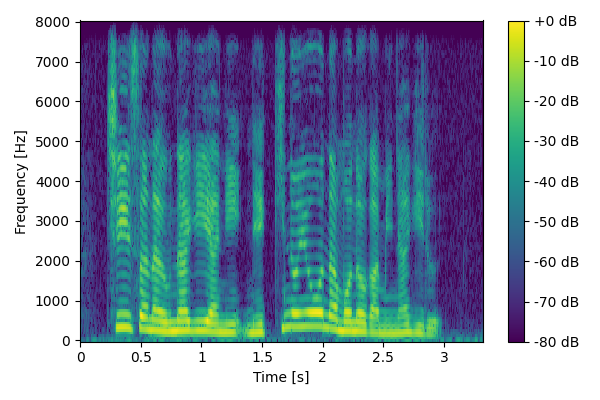
\includegraphics[width=\textwidth]{./figure/sec2/spectrogram_1.png}
        \caption{窓長12.5ms、シフト幅5ms}
        \label{sec2:fig:spectrogram1}
    \end{subfigure}
    \begin{subfigure}[b]{0.48\textwidth}
        \centering
        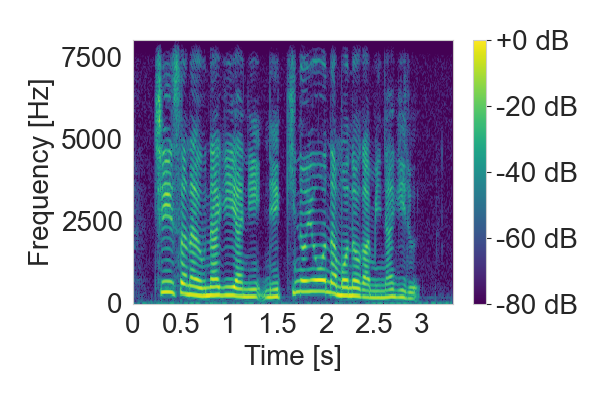
\includegraphics[width=\textwidth]{./figure/sec2/spectrogram_2.png}
        \caption{窓長25ms、シフト幅10ms}
        \label{sec2:fig:spectrogram2}
    \end{subfigure}

    \vspace{0.5cm}

    \begin{subfigure}[b]{0.48\textwidth}
        \centering
        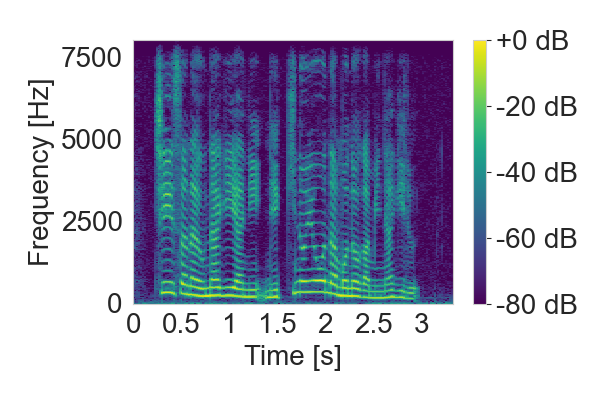
\includegraphics[width=\textwidth]{./figure/sec2/spectrogram_4.png}
        \caption{窓長50ms、シフト幅20ms}
        \label{sec2:fig:spectrogram3}
    \end{subfigure}
    \begin{subfigure}[b]{0.48\textwidth}
        \centering
        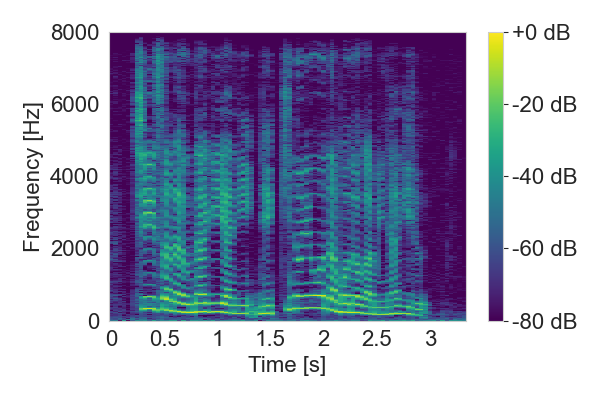
\includegraphics[width=\textwidth]{./figure/sec2/spectrogram_8.png}
        \caption{窓長100ms、シフト幅40ms}
        \label{sec2:fig:spectrogram4}
    \end{subfigure}
    \caption{「小さな鰻屋に、熱気のようなものがみなぎる」と発話した音声から計算された対数パワースペクトログラム}
    \label{sec2:fig:log_power_spectrograms}
\end{figure}

\subsection{メルスペクトログラム}
メルスペクトログラムは、パワースペクトログラムを人間の聴感特性を考慮したメル尺度に変換することによって得られる。周波数軸をメル尺度に変換する際、以下の式を用いる。
\begin{equation}
    \text{Mel}(f) = 2595\log_{10} \left(1 + \frac{f}{700}\right)
\end{equation}
メル尺度は、$\SI[]{1000}{Hz}$、$\SI[]{40}{dB}$の純音を$\SI[]{1000}{mel}$とする比率尺度である。メル尺度を用いることにより、低い周波数ほど細かく、高い周波数ほど荒い特徴量になる。メルスペクトログラムは、パワースペクトログラムに対してメルフィルタバンクを適用することによって得られる。メルフィルタバンクの数は任意に決定できるパラメータであり、メルスペクトログラムの周波数方向の次元はこれに一致する。音声合成においては、音声のサンプリング周波数を$\SI[]{16}{kHz}$とするとき、メルフィルタバンクの数を80とし、$\SI[]{8000}{Hz}$までの帯域に対して適用することが多い。「小さな鰻屋に、熱気のようなものがみなぎる」と発話した音声に対し、窓関数にハニング窓を用い、窓長25ms、シフト幅10msとしてパワースペクトログラムを計算した上で、80次元のメルフィルタバンクを適用して得られた対数メルスペクトログラムを、図~\ref{sec2:fig:melspectrogram}に示す。
\begin{figure}[bt]
    \centering
    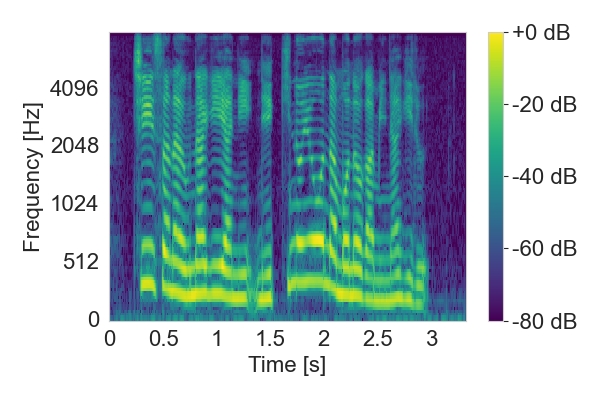
\includegraphics[height=70mm]{./figure/sec2/melspectrogram.png}
    \caption{「小さな鰻屋に、熱気のようなものがみなぎる」と発話した音声に対する対数メルスペクトログラム}
    \label{sec2:fig:melspectrogram}
\end{figure}

\clearpage

\section{深層学習}
深層学習とは、人間の神経細胞の仕組みを模擬したニューラルネットワークを用いる機械学習手法のことである。特に近年ではその層を深くしたディープニューラルネットワーク(Deep Neural Network; DNN)が用いられ、大量のパラメータによる表現力により、自然言語処理や画像処理、音声認識や音声合成など様々な分野で成果を上げている。本章では、本研究で使用するニューラルネットワーク及び、構築したDNNの学習方法について説明する。

\subsection{ニューラルネットワーク}
\subsubsection{全結合層}
全結合層は、すべての入力ノードがすべての出力ノードに接続される層である。全結合層の出力は、入力に対して学習可能な重みによる線形変換を適用することで得られる。入力$\bm{x} \in \mathbb{R}^{n}$に対し、出力$\bm{y} \in \mathbb{R}^{m}$は、
\begin{align}
    \bm{y} = \bm{W}\bm{x} + \bm{b}
\end{align}
で計算される。ここで、$\bm{W} \in \mathbb{R}^{m \times n}$は重み行列で、$\bm{b} \in \mathbb{R}^{m}$はバイアスベクトルである。全結合層は特徴量の次元の変換に用いられ、特に最終層において、ネットワークの特徴量を所望の特徴量の次元に変換する際に便利である。

\subsubsection{畳み込み層}
畳み込み層は、入力に対して畳み込み演算を行う層である。一次元畳み込み層について、入力$\bm{x} \in \mathbb{R}^{C_{\text{in}} \times T_{\text{in}}}$に対し、出力$\bm{y} \in \mathbb{R}^{C_{\text{out}} \times T_{\text{out}}}$は、$\bm{y}_{k}[i]$を出力テンソルの$k$番目のチャネルの$i$番目の成分とすると、
\begin{align}
    \bm{y}_{k}[i] = b_{k} + \sum_{c=0}^{C_{\text{in}} - 1} \sum_{m = 0}^{M - 1} \bm{x}_{c}\left[i - \left\lfloor \frac{M}{2} \right\rfloor + m\right] \bm{W}_{k, c}[m]
\end{align}
で計算される。ここで、$M$がカーネルサイズ、$\bm{x}_{c}\left[i - \left\lfloor \frac{M}{2} \right\rfloor + m\right]$が入力テンソルの$c$番目のチャネルの$\left[i - \left\lfloor \frac{M}{2} \right\rfloor + m\right]$番目の成分、$\bm{W}_{k, c}[m]$が出力チャネル$k$と入力チャネル$c$に対応するカーネルの$m$番目の成分である。上式より、一次元畳み込み層の$i$番目の出力は、$i$番目の入力を中心とし、カーネルサイズの範囲分が考慮されて得られる値だと解釈できる。一次元畳み込みは、自然言語や音声といった一次元系列に対する特徴抽出のために用いられることが多い。

これに加えて、カーネルを二次元配列とすれば二次元畳み込み層、三次元配列とすれば三次元畳み込み層となる。二次元畳み込み層は主に画像に用いられることが多く、三次元畳み込みは動画に用いられることが多い。

畳み込み層における主要なパラメータは三つある。一つ目は、カーネルサイズである。名のとおりカーネルのサイズであり、これによって考慮できる入力特徴量の範囲が定まる。二つ目は、ストライドである。この値はカーネルのシフト幅にあたる。三つ目は、ダイレーションである。これは畳み込み演算における入力特徴量の間隔を表す。ダイレーションを大きくすることによって、カーネルサイズが同じでも考慮できる範囲が広がることが特徴である。また、出力の系列長を入力に対して整数倍に保つためには、上記のパラメータに対して適切なパディング長を指定する必要がある。例えば、カーネルサイズを3、ストライドとダイレーションを1とした場合には、入力の両端に1ずつゼロパディングすることで入出力の系列長が保たれる。図~\ref{sec3:fig:conv_variations}に、ある入出力チャネル間における一次元畳み込み層の処理を示す。

\begin{figure}[tb]
    \centering
    \begin{subfigure}[b]{0.48\textwidth}
        \centering
        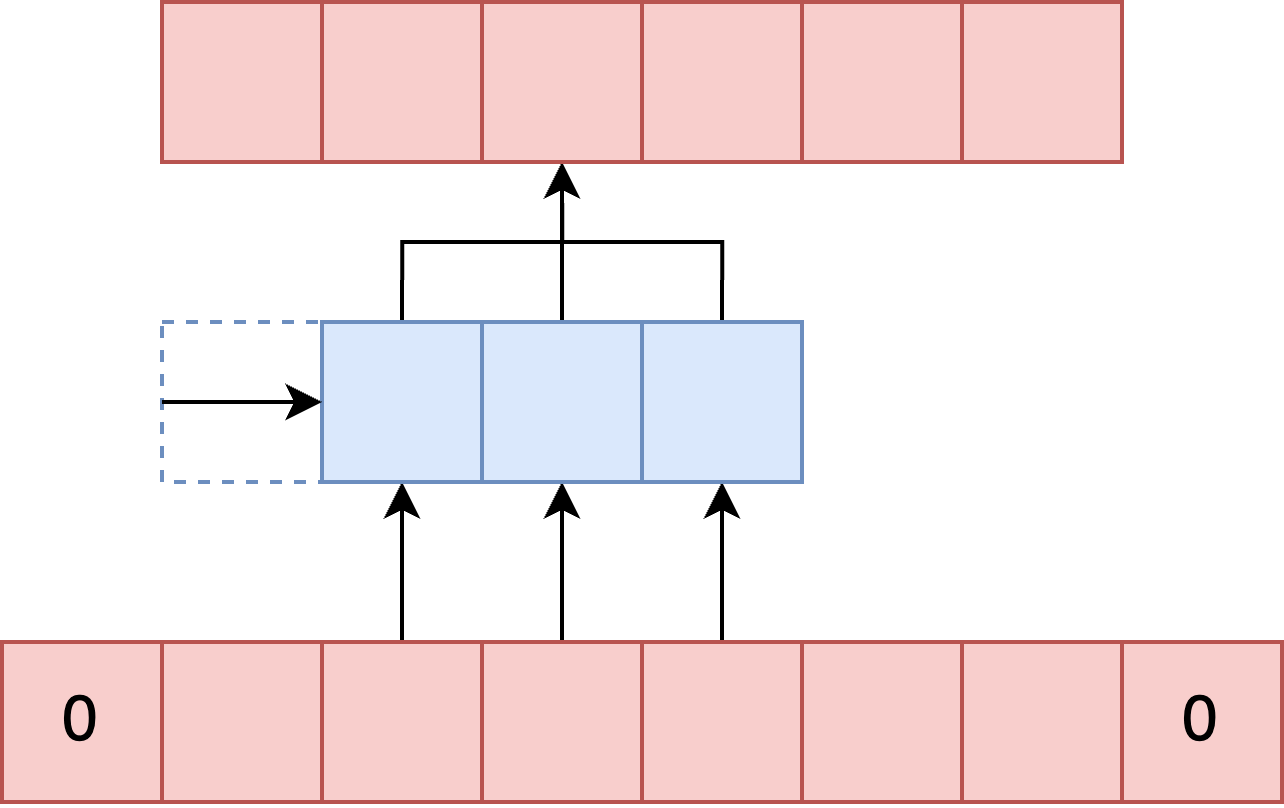
\includegraphics[height=4cm]{./figure/sec3/conv1.drawio.png}
        \caption{(k, s, d) = (3, 1, 1)}
        \label{sec3:fig:conv1}
    \end{subfigure}
    \begin{subfigure}[b]{0.48\textwidth}
        \centering
        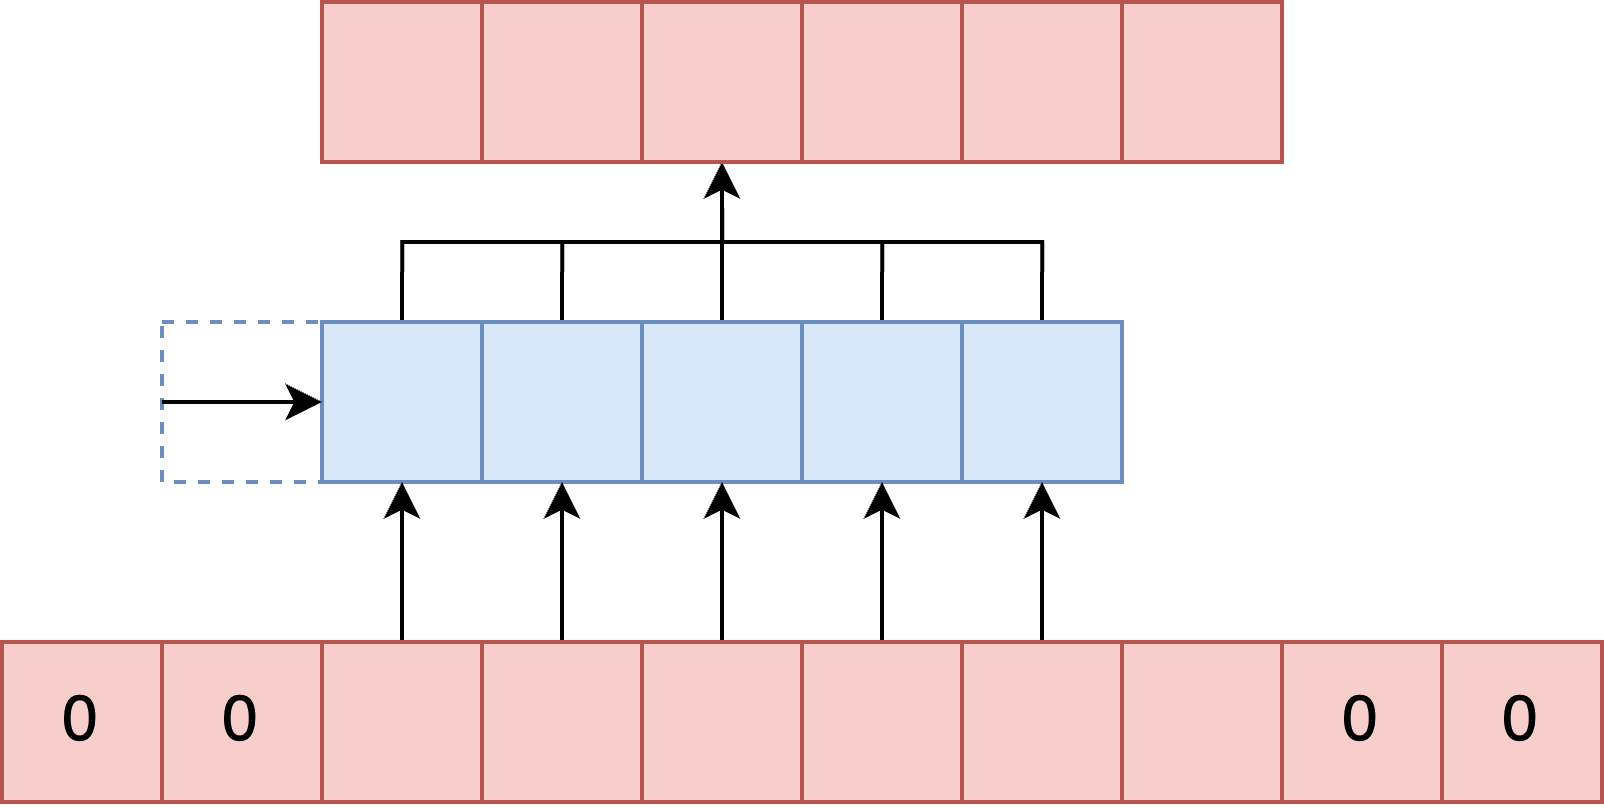
\includegraphics[height=4cm]{./figure/sec3/conv2.drawio.png}
        \caption{(k, s, d) = (5, 1, 1)}
        \label{sec3:fig:conv2}
    \end{subfigure}

    \vspace{0.5cm}

    \begin{subfigure}[b]{0.48\textwidth}
        \centering
        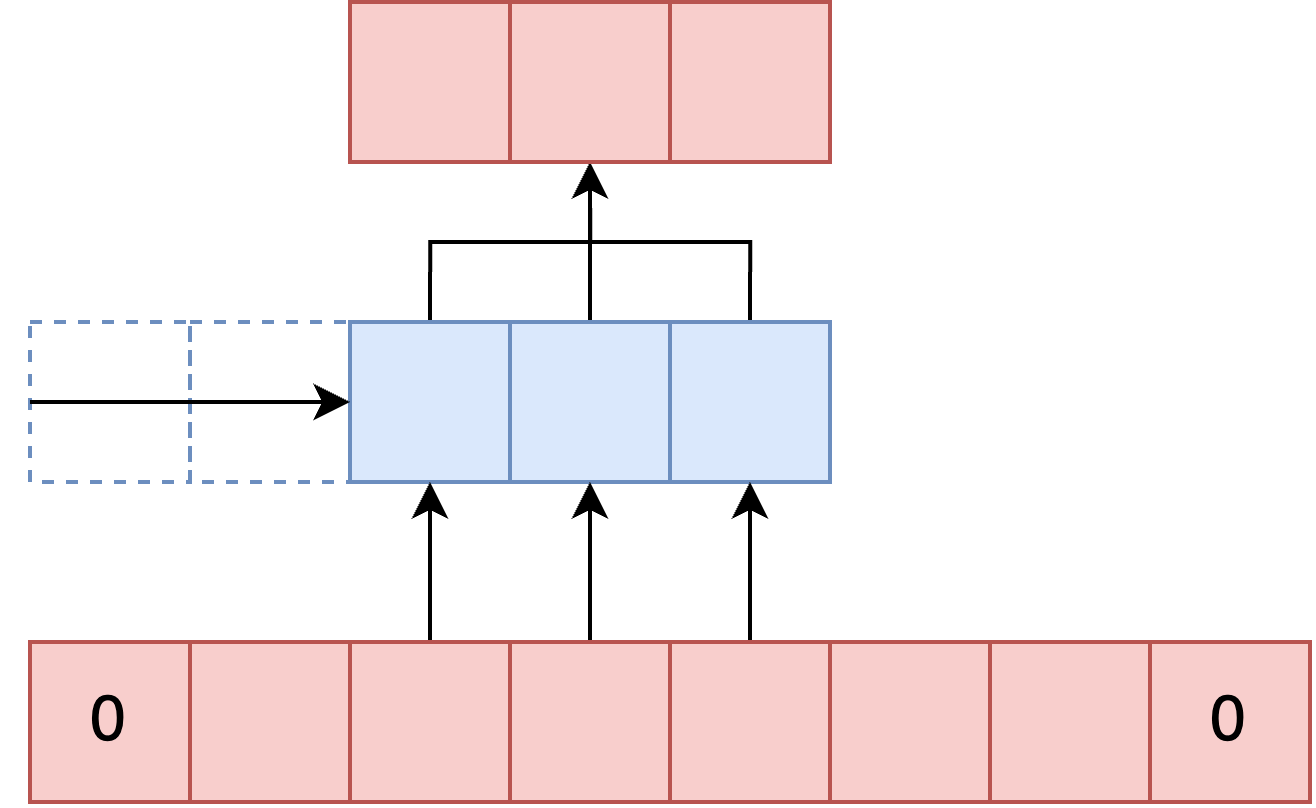
\includegraphics[height=4cm]{./figure/sec3/conv3.drawio.png}
        \caption{(k, s, d) = (3, 2, 1)}
        \label{sec3:fig:conv3}
    \end{subfigure}
    \begin{subfigure}[b]{0.48\textwidth}
        \centering
        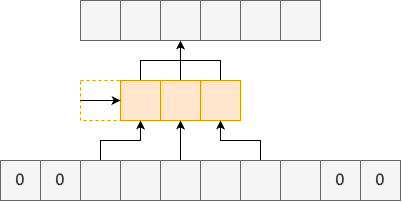
\includegraphics[height=4cm]{./figure/sec3/conv4.drawio.png}
        \caption{(k, s, d) = (3, 1, 2)}
        \label{sec3:fig:conv4}
    \end{subfigure}
    \caption{ある入出力チャネル間における一次元畳み込み層の処理。kはカーネルサイズ、sはストライド、dはダイレーションを表し、図中の0はパディング部。}
    \label{sec3:fig:conv_variations}
\end{figure}

\subsubsection{転置畳み込み層}
転置畳み込み層は、畳み込み層の逆演算に対応する層であり、主に入力のアップサンプリングに使用される。図~\ref{sec3:fig:tconv_variations}に、ある入出力チャネル間における一次元転置畳み込み層の処理を示す。転置畳み込み層では、$i$番目の入力とカーネルの積を計算し、その結果を$i$番目から$i + M - 1$番目までの出力とする。ここで$M$はカーネルサイズを表す。また、複数の入力から計算された出力がオーバーラップする場合、これらは加算される。図~\ref{sec3:fig:tconv1}は、カーネルサイズを4、ストライドを1とした場合の様子である。アップサンプリングを行いたい場合は、ストライドを2以上とすれば良い。図~\ref{sec3:fig:tconv2}にカーネルサイズを4、ストライドを2とした場合を示す。この時、入力系列長が4であるのに対して、出力系列長が10まで拡大されていることがわかる。ここで、出力系列長を入力系列長の整数倍に保つためには、パディングの値を適切に設定する必要がある。転置畳み込み層におけるパディングは、出力の両端の削除数である。上述の例ではパディングを1とすることで、出力系列長を入力系列長の2倍である8に調整できる。

\begin{figure}[tb]
    \centering
    \begin{subfigure}[b]{0.48\textwidth}
        \centering
        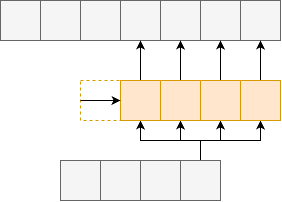
\includegraphics[height=4cm]{./figure/sec3/tconv1.drawio.png}
        \caption{(k, s) = (4, 1)}
        \label{sec3:fig:tconv1}
    \end{subfigure}
    \begin{subfigure}[b]{0.48\textwidth}
        \centering
        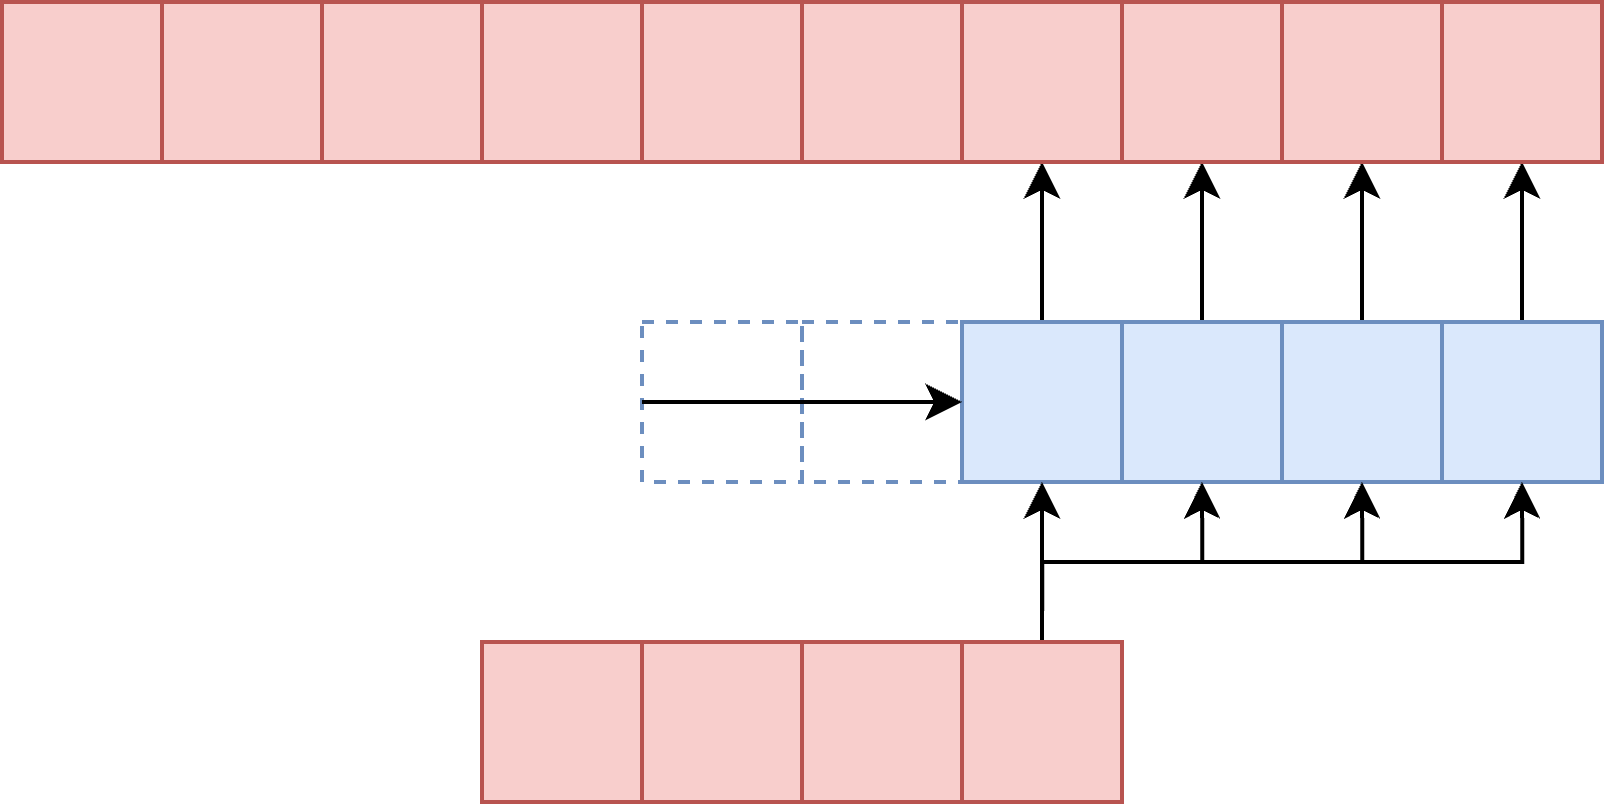
\includegraphics[height=4cm]{./figure/sec3/tconv2.drawio.png}
        \caption{(k, s) = (4, 2)}
        \label{sec3:fig:tconv2}
    \end{subfigure}
    \caption{ある入出力チャネル間における一次元転置畳み込み層の処理。kはカーネルサイズ、sはストライド。}
    \label{sec3:fig:tconv_variations}
\end{figure}
\subsubsection{活性化関数}
% 各関数について、具体的な用途が挙げられると良い。また、論文を読んで引用できるとさらに良い。
活性化関数は、ニューラルネットワークの出力に非線形性を与えるための関数である。これにより、DNNは単純な線形変換だけでは表現できない複雑な入出力の関係を学習可能になる。以下、活性化関数への入力を$x \in \mathbb{R}$として、代表的なものを述べる。また、活性化関数とその一階導関数のグラフを図~\ref{sec3:fig:activations_and_their_prime}に示す。

一つ目は、シグモイド関数である。シグモイド関数は
\begin{equation}
    \sigma(x) = \frac{1}{1 + \exp(-x)}
\end{equation}
で与えられ、その一階導関数は
\begin{equation}
    \frac{d}{dx}\sigma(x) = \frac{\exp(-x)}{(1 + \exp(-x))^{2}}
\end{equation}
となる。図~\ref{sec3:fig:activations_prime}より、シグモイド関数の一階導関数の最大値は$x=0$における0.25であり、入力が0から離れるほど微分係数が小さくなることが分かる。DNNの学習では、損失関数の重みに対する勾配を逆伝播する必要があり、これは合成関数の微分における連鎖律に従って行われる。シグモイド関数は取り得る微分係数の値が小さく、特に層数が深いDNNにおいては勾配が小さくスケーリングされていくことで、浅い層の重みに対する勾配のノルムが小さくなりすぎる可能性がある。この問題は、勾配消失と呼ばれる。

二つ目は、tanh関数である。tanh関数は
\begin{equation}
    \tanh(x) = \frac{\exp(x) - \exp(-x)}{\exp(x) + \exp(-x)}
\end{equation}
で与えられ、その一階導関数は
\begin{align}
    \frac{d}{dx}\tanh(x) & = \frac{4}{(\exp(x) + \exp(-x))^{2}} \\
                         & = \frac{1}{\cosh(x)^{2}}
\end{align}
となる。シグモイド関数と比較すると、シグモイド関数の値域が$[0, 1]$であったのに対し、tanh関数の値域は$[-1, 1]$となっている。シグモイド関数やtanh関数を実際に活性化関数として利用するニューラルネットワークとして、後述するLSTMやGRUが挙げられる。

三つ目は、ReLUである。ReLUは
\begin{equation}
    \text{ReLU}(x) = \max (0, x)
\end{equation}
で与えられ、その一階導関数は
\begin{equation}
    \frac{d}{dx}\text{ReLU}(x) =
    \begin{cases}
        1 & \text{if $x > 0$}  \\
        0 & \text{if $x <= 0$}
    \end{cases}
\end{equation}
となる。ReLUは入力が0以上であれば恒等写像となるが、0未満であれば0に写す。一階導関数は0あるいは1のみを取り、特に入力が正の値であれば常に微分係数は1となることから、シグモイド関数よりも勾配消失問題が起こりづらくなっている。ReLUは現在、標準的な活性化関数として広く用いられている。
% 一方、ReLUは0以下の入力に対して微分係数が0となるため、勾配も0となる。従って、入力が負の値に偏った場合には勾配が0になり続け、重みの更新が進まなくなる可能性がある。この問題を、Dying ReLU問題と呼ぶ。

% 四つ目は、LeakyReLUである。LeakyReLUは
% \begin{equation}
%     \text{LeakyReLU}(x) =
%     \begin{cases}
%         x  & \text{if $x > 0$}  \\
%         ax & \text{if $x <= 0$}
%     \end{cases}
% \end{equation}
% で与えられ、その一階導関数は
% \begin{equation}
%     \frac{d}{dx}\text{LeakyReLU}(x) =
%     \begin{cases}
%         1 & \text{if $x > 0$}  \\
%         a & \text{if $x <= 0$}
%     \end{cases}
% \end{equation}
% となる。ここで、aはnegative slopeと呼ばれるパラメータである。ReLUと比較すると、0以下の入力に対しても0でない値を取り、また微分係数も0にならない点が異なっている。この工夫により、勾配が0になり続ける恐れがなくなるため、前述したDying ReLU問題に対処することが可能である。具体的な利用ケースとしては、敵対的生成ネットワーク(Generative adversarial network; GAN)におけるGeneratorやDiscriminatorが挙げられる。

% 五つ目は、PReLUである。これは四つ目に述べたLeakyReLUと非常に似た活性化関数であるが、LeakyReLUのnegative slopeを学習可能なパラメータに変更したという点で異なっている。

% 六つ目は、GELUである。GELUは
% \begin{equation}
%     \text{GELU}(x) = x \Phi(x)
% \end{equation}
% で与えられる。ここで、$\Phi(x)$は標準正規分布の累積分布関数である。GELUの一階導関数は、
% \begin{equation}
%     \frac{d}{dx}\text{GELU}(x) = \Phi(x) + \frac{x}{\sqrt{2\pi}}\exp(-\frac{x^{2}}{2})
% \end{equation}
% となる。GELUは入力に対して標準正規分布に基づく確率値を利用したスケーリングを行う活性化関数であり、後述するTransformerなど大規模なモデルにおいて採用される場合がある。

\begin{figure}[tb]
    \centering
    \begin{subfigure}[b]{1.0\textwidth}
        \centering
        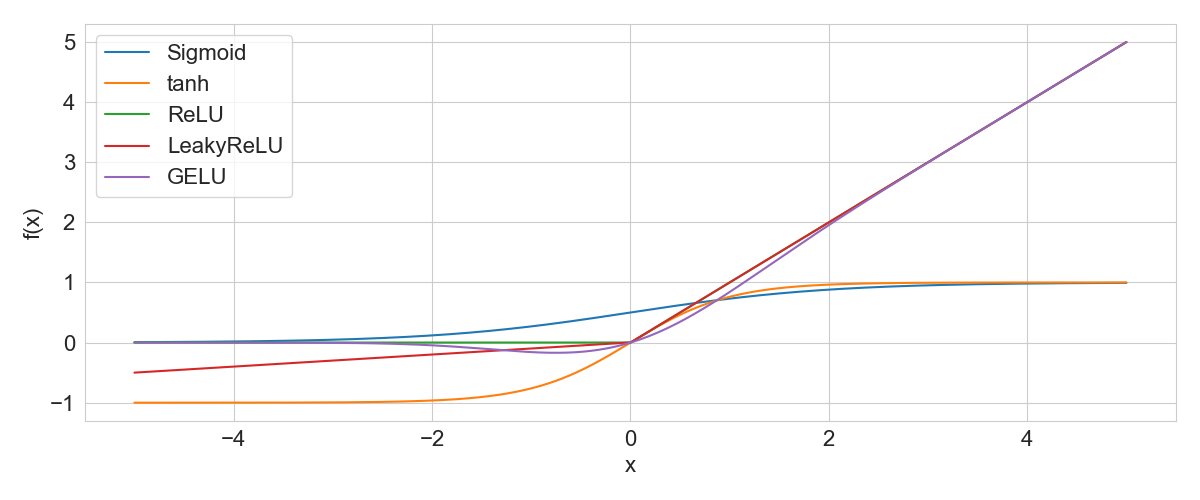
\includegraphics[height=6cm]{./figure/sec3/activations.png}
        \caption{活性化関数}
        \label{sec3:fig:activations}
    \end{subfigure}
    \begin{subfigure}[b]{1.0\textwidth}
        \centering
        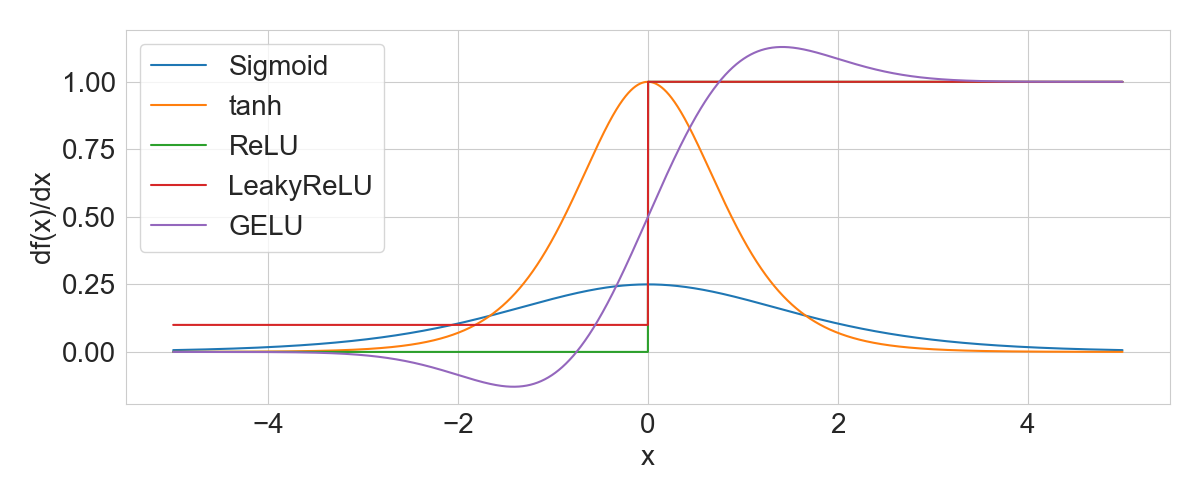
\includegraphics[height=6cm]{./figure/sec3/activations_prime.png}
        \caption{活性化関数の一階導関数}
        \label{sec3:fig:activations_prime}
    \end{subfigure}
    \caption{活性化関数の例}
    \label{sec3:fig:activations_and_their_prime}
\end{figure}

\subsubsection{再帰型ニューラルネットワーク}
再帰型ニューラルネットワーク(Recurrent Neural Network; RNN)は、自身の過去の出力を保持し、それをループさせる再帰的な構造を持ったネットワークである。

近年よく用いられるRNNとして、長・短期記憶(Long Short-Time Memory; LSTM)\cite{hochreiter1997long}がある。LSTMでは入力ゲート、忘却ゲート、出力ゲートの3つを持ち、これらゲートによってネットワーク内部の情報の取捨選択を行うことで、長い系列データからの学習を可能にした。LSTMのネットワーク内部で行われる計算を以下に示す。
\begin{gather}
    \bm{f}_{t} = \sigma(\bm{W}_{f}[\bm{x}_{t}, \bm{h}_{t-1}] + \bm{b}_{f}) \\
    \bm{i}_{t} = \sigma(\bm{W}_{i}[\bm{x}_{t}, \bm{h}_{t-1}] + \bm{b}_{i}) \\
    \tilde{\bm{c}_{t}} = \tanh (\bm{W}_{h}[\bm{x}_{t}, \bm{h}_{t-1}] + \bm{b}_{h}) \\
    \bm{c}_{t} = \bm{f}_{t} \odot \bm{c}_{t-1} + \bm{i}_{t} \odot \tilde{\bm{c}_{t}} \\
    \bm{o}_{t} = \sigma(\bm{W}_{o}[\bm{x}_{t}, \bm{h}_{t-1}] + \bm{b}_{o}) \\
    \bm{h}_{t} = \bm{o}_{t} \odot \tanh(\bm{c}_{t})
\end{gather}
ここで、$\bm{x}_{t} \in \mathbb{R}^{n}$は時刻$t$の入力、$\bm{f}_{t} \in [0, 1]^{m}$は忘却ゲートの出力、$\bm{i}_{t} \in [0, 1]^{m}$は入力ゲートの出力、$\bm{c}_{t} \in [-1, 1]^{m}$が時刻$t$におけるセルの状態、$\bm{o}_{t} \in [0, 1]^{m}$が出力ゲートの出力、$\bm{h}_{t} \in [-1, 1]^{m}$が時刻$t$における隠れ状態を表す。また、$[\cdot, \cdot]$は次元方向の結合演算子、$\odot$は要素積を表す。$\bm{W}_{f}, \bm{W}_{i}, \bm{W}_{h}, \bm{W}_{o} \in \mathbb{R}^{m \times (n + m)}$は学習可能な重み行列、$\bm{b}_{f}, \bm{b}_{i}, \bm{b}_{h}, \bm{b}_{o} \in \mathbb{R}^{m}$は学習可能なバイアスベクトルである。忘却ゲートの出力$\bm{f}_{t}$は、前時刻のセル状態$\bm{c}_{t-1}$との要素積に用いられ、これによってネットワーク内に保持されていた長期記憶に対して忘却するべき情報を与え、取捨選択を行う。入力ゲートの出力$\bm{i}_{t}$は時刻$t$のセル状態の候補となる$\tilde{\bm{c}_{t}}$との要素積に用いられ、これによって新たにネットワークが長期記憶するべき情報が選択され、セル状態$\bm{c}_{t}$として保持される。出力ゲートの出力$\bm{o}_{t}$は時刻$t$のセル状態$\bm{c}_{t}$に$\tanh$を適用した値との要素積に用いられ、これによって時刻$t$において出力するべき情報を選択する。最後に、隠れ状態$\bm{h}_{t}$は、時刻$t$の出力と$\tanh$を適用したセル状態$\bm{c}_{t}$から決定される。このように、$\bm{h}_{t}$及び$\bm{c}_{t}$を入力に対して適応的に変化させながら情報を取捨選択することで、長い系列長のデータに対しての学習を可能にした。

また、LSTMでは3つのゲートを必要とするが、ゲートを2つに減らすことでネットワークの軽量化を図ったネットワークとして、ゲート付き回帰型ユニット(Gated Recurrent Unit; GRU)\cite{cho2014learning}がある。GRUではリセットゲートと更新ゲートの2つのゲートを用いて隠れ状態$\bm{h}_{t}$を再帰的に更新する。また、LSTMと違ってセル状態$\bm{c}_{t}$を省いており、よりシンプルな構造となっている。GRUのネットワーク内部で行われる計算を以下に示す。
\begin{gather}
    \bm{z}_{t} = \sigma(\bm{W}_{z}[\bm{x}_{t}, \bm{h}_{t-1}] + \bm{b}_{z}) \\
    \bm{r}_{t} = \sigma(\bm{W}_{r}[\bm{x}_{t}, \bm{h}_{t-1}] + \bm{b}_{r}) \\
    \tilde{\bm{h}_{t}} = \tanh(\bm{W}_{h}[\bm{x}_{t}, \bm{r}_{t} \odot \bm{h}_{t-1}] + \bm{b}_{h}) \\
    \bm{h}_{t} = (1 - \bm{z}_{t}) \odot \bm{h}_{t-1} + \bm{z}_{t} \odot \tilde{\bm{h}_{t}}
\end{gather}
ここで、$\bm{x}_{t} \in \mathbb{R}^{n}$が時刻$t$における入力、$\bm{z}_{t} \in [0, 1]^{m}$が更新ゲートの出力、$\bm{r}_{t} \in [0, 1]^{m}$がリセットゲートの出力、$\bm{h}_{t} \in [-1, 1]^{m}$が時刻$t$における隠れ状態を表す。また、$\bm{W}_{z}, \bm{W}_{r}, \bm{W}_{h} \in \mathbb{R}^{m \times (n + m)}$は学習可能な重み行列、$\bm{b}_{z}, \bm{b}_{r}, \bm{b}_{h} \in \mathbb{R}^{m}$は学習可能なバイアスベクトルである。更新ゲートの出力$\bm{z}_{t}$はネットワーク内で新たに記憶するべき情報の割合を決定する役割を果たす。一方、リセットゲートの出力$\bm{r}_{t}$は前時刻の隠れ状態$\bm{h}_{t-1}$との要素積に用いられ、これによって忘却するべき情報が選択される。リセットゲートの出力によって処理された内部表現から、時刻$t$の隠れ状態の候補となる$\tilde{\bm{h}_{t}}$が計算される。最後に、前時刻の隠れ状態$\bm{h}_{t-1}$と隠れ状態の候補$\tilde{\bm{h}_{t}}$に対して更新ゲートの出力$\bm{z}_{t}$を用いた重み付け和を計算することで、隠れ状態$\bm{h}_{t}$を決定する。

\subsubsection{Transformer}
Transformer\cite{vaswani2017attention}は、自己注意機構(Self-Attention)を用いて、入力系列全体に渡る依存関係を捉えることができるニューラルネットワークである。特に、再帰的な計算を必要とするRNNと比較して、Transformerは並列計算のみ行うため、GPUによる計算の高速化が可能である。Transformerの内部構造について説明するため、入力系列$\bm{X} \in \mathbb{R}^{T \times d_{\text{model}}}$をとる。ここで、$T$は入力系列の系列長、$d_{\text{model}}$は入力系列の次元である。また、Transformer層の構造を図~\ref{sec3:fig:transformer_layer}に示す。

\begin{figure}[bt]
    \centering
    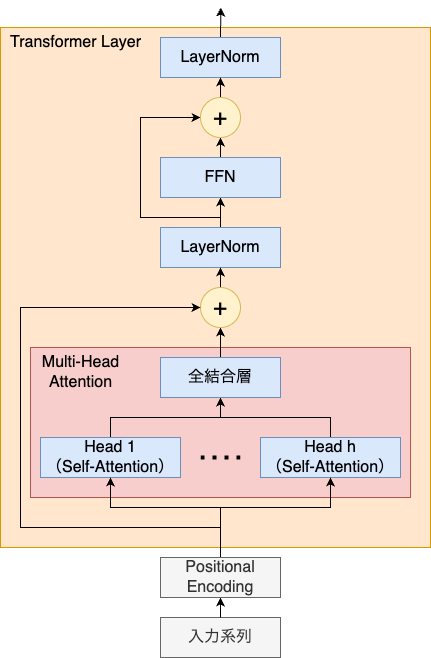
\includegraphics[height=140mm]{./figure/sec3/transformer.drawio.png}
    \caption{Transformer層の構造}
    \label{sec3:fig:transformer_layer}
\end{figure}

まず、クエリ$\bm{Q} \in \mathbb{R}^{T \times d_{k}}$、キー$\bm{K} \in \mathbb{R}^{T \times d_{k}}$、バリュー$\bm{V} \in \mathbb{R}^{T \times d_{v}}$の計算を行う。これは、
\begin{align}
    \bm{Q} & = \bm{X}\bm{W}_{Q} \\
    \bm{K} & = \bm{X}\bm{W}_{K} \\
    \bm{V} & = \bm{X}\bm{W}_{V}
\end{align}
で与えられる。ここで、$d_{k}$はキーとクエリの次元、$d_{v}$はバリューの次元、$\bm{W_{Q}} \in \mathbb{R}^{d_{\text{model}} \times d_{k}}$はクエリに対する重み行列、$\bm{W_{K}} \in \mathbb{R}^{d_{\text{model}} \times d_{k}}$はキーに対する重み行列、$\bm{W_{V}} \in \mathbb{R}^{d_{\text{model}} \times d_{v}}$はバリューに対する重み行列である。次に、クエリ$\bm{Q}$とキー$\bm{K}$を元にアテンション重みを求め、バリューに対する行列積を計算する。
\begin{equation}
    \text{Attention}(\bm{Q}, \bm{K}, \bm{V}) = \text{softmax}\left(\frac{\bm{Q}\bm{K}^\top}{\sqrt{d_{k}}}\right) \bm{V}
\end{equation}
で与えられる。式中の$\bm{Q}\bm{K}^\top \in \mathbb{R}^{T \times T}$について、この行列の$(i, j)$成分$(\bm{Q}\bm{K}^\top)_{i, j}$は、クエリベクトル$\bm{Q}_{i} \in \mathbb{R}^{d_{k}}$と、キーベクトル$\bm{K}_{j} \in \mathbb{R}^{d_{k}}$の内積であり、$\bm{Q}_{i}$と$\bm{K}_{i}$の関連度を表していると解釈できる。また、softmax関数が行方向に適用されることで、$i$番目のクエリベクトル$\bm{Q}_{i}$から$\bm{K}_{j} ~ (j = 1, \ldots, T)$に対する注意度が、確率分布として表されていると解釈できる。
最後にアテンション重み$\text{softmax}\left(\bm{Q}\bm{K}^\top / \sqrt{d_{k}}\right)$をバリュー$\bm{V}$にかけることにより、各バリューベクトル$\bm{V}_{i} \in \mathbb{R}^{d_{v}}$は、$\bm{Q}_{i}$からキーへの注意度による重み付け和となる。

Transformerでは、Self-Attentionを複数のヘッドで並列に計算し、各ヘッドの出力を結合して最終出力を得るMulti-Head Attentionが用いられる。ヘッド数を$H$とすると、各ヘッド$h$におけるクエリ$\bm{Q}^{h} \in \mathbb{R}^{T \times \frac{d_{k}}{H}}$、キー$\bm{K}^{h} \in \mathbb{R}^{T \times \frac{d_{k}}{H}}$、バリュー$\bm{V}^{h} \in \mathbb{R}^{T \times \frac{d_{v}}{H}}$の計算は、
\begin{align}
    \bm{Q}^{h} & = \bm{X}\bm{W}_{Q}^{h} \\
    \bm{K}^{h} & = \bm{X}\bm{W}_{K}^{h} \\
    \bm{V}^{h} & = \bm{X}\bm{W}_{V}^{h}
\end{align}
で与えられる。ここで、$\bm{W}_{Q}^{h} \in \mathbb{R}^{d_{\text{model}} \times \frac{d_{k}}{H}}$は$h$番目のヘッドのクエリに対する重み行列、$\bm{W}_{K}^{h} \in \mathbb{R}^{d_{\text{model}} \times \frac{d_{k}}{H}}$は$h$番目のヘッドのキーに対する重み行列、$\bm{W}_{V}^{h} \in \mathbb{R}^{d_{\text{model}} \times \frac{d_{v}}{H}}$は$h$番目のヘッドのバリューに対する重み行列である。この後の処理も同様に、
\begin{equation}
    \text{Attention}(\bm{Q}^{h}, \bm{K}^{h}, \bm{V}^{h}) = \text{softmax}\left(\frac{\bm{Q}^{h}(\bm{K}^{h})^\top}{\sqrt{d_{k}} / H}\right) \bm{V}^{h}
\end{equation}
で行われる。その後、すべてのヘッドからの出力を結合し、さらに線形変換を適用することでMulti-Head Attetionの出力が得られる。これは、
\begin{equation}
    \text{MultiHead}(\bm{Q}, \bm{K}, \bm{V}) = \text{Concat}(\text{head}^{1}, \ldots, \text{head}^{H})\bm{W}_{o}
\end{equation}
と表される。ここで、$\text{head}^{h} \in \mathbb{R}^{T \times \frac{d_{v}}{H}}$が各ヘッドから出力されたAttentionスコア、$\text{Concat}(\text{head}^{1}, \\ \ldots, \text{head}^{H}) \in \mathbb{R}^{T \times d_{v}}$が全ヘッドのAttentionスコアを結合した特徴量、$\bm{W}_{o} \in \mathbb{R}^{d_{v} \times d_{\text{model}}}$が最終的な線形変換に用いられる重み行列である。ヘッドを分割することで複数パターンのアテンションが可能になり、これが入出力間の複雑な関係性を考慮するのに役立っていると考えられる。Multi-Head Attention後には、残差結合と後述するレイヤー正規化を適用する。
これは、出力系列を$\bm{Y} \in \mathbb{R}^{T \times d_{\text{model}}}$とすると、
\begin{equation}
    \bm{Y} = \text{LayerNorm}\left(\text{MultiHead}(\bm{Q}, \bm{K}, \bm{V}) + \bm{X}\right)
\end{equation}
で与えられる。

Multi-Head Attentionによって系列全体の依存関係を考慮した後は、各フレームごとに独立して全結合層を適用する。これは、
\begin{equation}
    \text{FFN}(\bm{Y}) = \text{ReLU}(\bm{Y}\bm{W}_{1} + \bm{b}_{1})\bm{W}_{2} + \bm{b}_{2}
\end{equation}
で与えられる。
ここで、$\bm{W}_{1} \in \mathbb{R}^{d_{\text{model}} \times d_{\text{ff}}}$、$\bm{W}_{2} \in \mathbb{R}^{d_{1} \times d_{\text{model}}}$は学習可能な重み行列、$\bm{b}_{1} \in \mathbb{R}^{d_{\text{ff}}}$、$\bm{b}_{2} \in \mathbb{R}^{d_{\text{model}}}$はバイアスベクトルである。$d_{\text{ff}}$は$d_{\text{model}}$の4倍とされることが多い。全結合層適用後は、Multi-Head Attention後と同様に、残差結合とレイヤー正規化を適用する。

上述したMulti-Head Attentionとフレームごとに適用される全結合層を合わせて、Transformer層と呼ぶ。実際には、Transformer層を多層積み重ねて用いることが多い。

最後に、TransformerではRNNと違い、並列計算によって系列全体を一度に処理することが可能であるが、それと引き換えに入力の順序情報を考慮することができなくなる。この問題に対し、入力系列に対して位置情報を与えるために行われるのが、Positional Encodingである。Positional Encodingは$\sin$関数と$\cos$関数に基づいて計算される値であり、
\begin{align}
    \text{PE}_{\text{pos}, 2d}     & = \sin \left(\frac{\text{pos}}{10000^{2d / d_{\text{model}}}}\right) \\
    \text{PE}_{\text{pos}, 2d + 1} & = \cos \left(\frac{\text{pos}}{10000^{2d / d_{\text{model}}}}\right)
\end{align}
で与えられる。ここで、$\text{pos}$は入力系列の位置を表し、$d$は入力系列の次元を表す。

\subsection{学習方法}
\subsubsection{損失関数}
損失関数は、DNNによって推定された結果と、正解値との間の誤差を求める関数のことであり、扱う問題によって様々である。例えば、回帰問題において用いられる関数の一つに、MAE(Mean Absolute Error) Lossがある。推定対象を$\bm{Y} \in \mathbb{R}^{T \times D}$、DNNによる推定結果を$\hat{\bm{Y}} \in \mathbb{R}^{T \times D}$とすると、MAE Lossは
\begin{equation}
    L_{MAE}(\bm{Y}, \hat{\bm{Y}}) = \frac{1}{TD} \sum_{t = 1}^{T} \sum_{d = 1}^{D}  |\bm{Y}_{t, d} - \hat{\bm{Y}}_{t, d}|
\end{equation}
で与えられる。ここで、$T$が系列長、$D$が次元である。

一方、分類問題において用いられる関数の一つに、Cross Entropy Lossがある。Cクラス分類の問題について、推定対象を$\bm{y} \in [0, 1]^{C}$、DNNによる推定結果を$\hat{\bm{y}} \in [0, 1]^{C}$とすると、Cross Entropy Lossは
\begin{equation}
    L_{CE}(\bm{y}, \hat{\bm{y}}) = - \sum_{c = 1}^{C} \bm{y}_{c}\log(\hat{\bm{y}}_{c})
\end{equation}
で与えられる。ここで、$\bm{y}, \hat{\bm{y}}$はどちらもクラスに対する確率分布であり、
\begin{equation}
    \sum_{c = 1}^{C} \bm{y}_{c} = 1, \quad \sum_{c = 1}^{C} \hat{\bm{y}}_{c} = 1
\end{equation}
を満たす。また、推定対象がテキストなどの系列長の次元を持ったテンソルとなる場合、推定対象を$\bm{Y} \in [0, 1]^{T \times C}$、DNNによる推定結果を$\hat{\bm{Y}} \in [0, 1]^{T \times C}$とすると、Cross Entropy Lossは
\begin{equation}
    L_{CE}(\bm{Y}, \hat{\bm{Y}}) = - \frac{1}{T} \sum_{t = 1}^{T} \sum_{c = 1}^{C} \bm{Y}_{t, c}\log(\hat{\bm{Y}}_{t, c})
\end{equation}
で与えられる。ここで、$\bm{Y}_{t}, \hat{\bm{Y}}_{t} \in [0, 1]^{C} ~ (t = 1, \ldots, T)$はそれぞれクラスに対する確率分布である。実際の分類問題において推定対象は、正解となるクラスのみを1、それ以外を0としたOne-hotベクトルとされることが多い。

\subsubsection{勾配降下法}
\label{sec3:sec:gradient_descent}
勾配降下法は、損失関数を最小化するDNNの重みとバイアスを得るための最適化手法である。モデルの重みとバイアスをまとめて$\bm{\theta}$、損失関数を$L(\bm{\theta})$とすると、勾配降下法による$\bm{\theta}$の更新は
\begin{equation}
    \bm{\theta} \leftarrow \bm{\theta} - \eta \nabla L(\bm{\theta})
\end{equation}
で表される。ここで、$\eta$は学習率と呼ばれるパラメータであり、$\bm{\theta}$の一回の更新による変化量を制御する役割を果たす。上式より、勾配降下法は損失関数の$\bm{\theta}$についての勾配を利用し、損失関数の値をより小さくする方向へ$\bm{\theta}$を更新する手続きを繰り返すことによって、損失関数の値を最小化するDNNを得ようとする最適化手法だと解釈できる。

勾配降下法には三種類の方法がある。一つ目は、バッチ勾配降下法である。これは、$\bm{\theta}$の更新一回につき、全学習データを利用して損失関数の勾配を計算する方法である。データ一つ一つのノイズに影響を受けづらく安定した更新が期待できるが、一回の更新にかかる計算コストが大きいというデメリットがある。二つ目は、確率的勾配降下法である。これは、$\bm{\theta}$の更新一回につき、ある一つの学習データのみによって損失関数の勾配を計算する方法である。バッチ勾配降下法と比較して一回の更新にかかる計算コストは低くなるが、各データのノイズによる影響が大きくなることで学習が不安定になる可能性がある。三つ目は、ミニバッチ勾配降下法である。これは、$\bm{\theta}$の更新一回につき、学習データの中から指定した個数のデータをサンプリングしてミニバッチを作成し、これを利用して損失関数の勾配を計算する方法である。ここで、サンプリングするデータの個数はバッチサイズと呼ばれる。ミニバッチ勾配降下法は、バッチ勾配降下法と確率的勾配降下法の間をとったような方法であり、バッチサイズによって一回の更新に利用するデータの数を調整可能であることが両者にないメリットである。実際、DNNの学習においてはミニバッチ勾配降下法が用いられることが多い。

\subsubsection{誤差逆伝播法}
\label{sec3:sec:backpropagation}
前述した勾配降下法によるDNNの最適化のためには、各重み及びバイアスについての損失関数の勾配を計算する必要があり、これは、微分の連鎖律に基づいて計算することが可能である。ここで、誤差逆伝播法は、各重み及びバイアスについての損失関数の勾配を、出力から入力へとDNNを遡る方向に再帰的に計算するアルゴリズムである。ここでは例として、全結合層と活性化関数のみからなる$L$層のDNNを構築し、ミニバッチ勾配降下法によって最適化する場面を考える。

まず、$\bm{W}_{i, j}^{k} \in \mathbb{R}$を$k - 1$層目の$i$番目のノードから$k$層目の$j$番目のノードに割り当てられた重み、$\bm{b}_{i}^{k} \in \mathbb{R}$を$k$層目の$i$番目のノードに割り当てられたバイアスとすると、$k$層目の$i$番目のノードにおける出力$\bm{a}_{i}^{k} \in \mathbb{R}$は、
\begin{equation}
    \label{sec3:eq:output_before_act}
    \bm{a}_{i}^{k} = \bm{b}_{i}^{k} + \sum_{j = 1}^{N_{k - 1}} \bm{W}_{j, i}^{k} \bm{o}_{j}^{k - 1}
\end{equation}
で与えられる。ここで、$N_{k - 1}$は$k - 1$層目の全結合層のチャンネル数、$\bm{o}_{j}^{k - 1} \in \mathbb{R}$は$k - 1$層目の$j$番目のノードにおける出力$\bm{a}_{j}^{k - 1}$に活性化関数$f$を適用した結果を表す。すなわち、
\begin{equation}
    \bm{o}_{j}^{k - 1} = f(\bm{a}_{j}^{k - 1})
\end{equation}
で与えられる。ここで、式~\eqref{sec3:eq:output_before_act}に対し、$\bm{W}_{0, i}^{k} = \bm{b}_{i}^{k}$とし、$\bm{o}_{0}^{k - 1} = 1$とすれば、
\begin{equation}
    \label{sec3:eq:output_before_act_2}
    \bm{a}_{i}^{k} = \bm{b}_{i}^{k} + \sum_{j = 1}^{N_{k - 1}} \bm{W}_{j, i}^{k} \bm{o}_{j}^{k - 1}
    = \sum_{j = 0}^{N_{k - 1}} \bm{W}_{j, i}^{k} \bm{o}_{j}^{k - 1}
\end{equation}
と整理できる。

次に、DNNの学習用データセットを$\{(\bm{x}_{n}, \bm{y}_{n})\}_{n = 1}^{N}$とおく。ここで、$N$はデータの数、$\bm{x}_{n} \in \mathbb{R}^{d_{x}}$はDNNへの入力ベクトル、$\bm{y}_{n} \in \mathbb{R}^{d_{y}}$は$\bm{x}_{n}$に対するDNNの推定対象を表す。さらに、DNNの推定結果を$\hat{\bm{y}}_{n} \in \mathbb{R}^{d_{y}}$とし、損失関数の値を$L(\bm{y_{n}}, \hat{\bm{y}}_{n} ; \bm{\theta})$とする。ここで、$\bm{\theta}$はDNNの全ての重みとバイアスをまとめて表した変数である。この時、ミニバッチ勾配降下法におけるバッチサイズを$N_{\text{batch}}$とすると、あるミニバッチにおける損失関数の重み$\bm{W}_{i, j}^{k}$についての勾配は、
\begin{align}
    \frac{\partial L}{\partial \bm{W}_{i, j}^{k}} & = \frac{\partial}{\partial \bm{W}_{i, j}^{k}} \left(\frac{1}{N_{\text{batch}}} \sum_{n = 1}^{N_{\text{batch}}} L(\bm{y_{n}}, \hat{\bm{y}}_{n}; \bm{\theta})\right) \\
                                                  & = \frac{1}{N_{\text{batch}}} \sum_{n = 1}^{N_{\text{batch}}} \frac{\partial}{\partial \bm{W}_{i, j}^{k}} L(\bm{y_{n}}, \hat{\bm{y}}_{n}; \bm{\theta})              \\
                                                  & = \frac{1}{N_{\text{batch}}} \sum_{n = 1}^{N_{\text{batch}}} \frac{\partial L_{n}}{\partial \bm{W}_{i, j}^{k}} \label{sec3:eq:loss_sample_wise_grad_sum}
\end{align}
となる。ここで、式~\eqref{sec3:eq:loss_sample_wise_grad_sum}では$L(\bm{y_{n}}, \hat{\bm{y}}_{n}; \bm{\theta}) = L_{n}$とおいた。式~\eqref{sec3:eq:loss_sample_wise_grad_sum}より、ミニバッチ全体における損失関数の勾配は、サンプルごとに計算される勾配の平均値であることがわかる。ここで、$\partial L_{n} / \partial \bm{W}_{i, j}^{k}$は、
\begin{equation}
    \label{sec3:eq:loss_sample_wise_grad}
    \frac{\partial L_{n}}{\partial \bm{W}_{i, j}^{k}} = \frac{\partial L_{n}}{\partial \bm{a}_{j}^{k}} \frac{\partial \bm{a}_{j}^{k}}{\partial \bm{W}_{i, j}^{k}}
\end{equation}
となる。ここで、式~\eqref{sec3:eq:output_before_act_2}より
\begin{equation}
    \frac{\partial \bm{a}_{j}^{k}}{\partial \bm{W}_{i, j}^{k}} = \frac{\partial}{\partial \bm{W}_{i, j}^{k}} \left( \sum_{l = 0}^{N_{k - 1}} \bm{W}_{l, j}^{k} \bm{o}_{l}^{k - 1} \right) = \bm{o}_{i}^{k - 1}
\end{equation}
であり、
\begin{equation}
    \delta_{j}^{k} = \frac{\partial L_{n}}{\partial \bm{a}_{j}^{k}}
\end{equation}
とおけば、式~\eqref{sec3:eq:loss_sample_wise_grad}は
\begin{equation}
    \frac{\partial L_{n}}{\partial \bm{W}_{i, j}^{k}} = \delta_{j}^{k} \bm{o}_{i}^{k - 1}
\end{equation}
と書ける。ここで、まず出力層の重み$\bm{W}_{i, j}^{L}$についての$L_{n}$の勾配は、
\begin{align}
    \frac{\partial L_{n}}{\partial \bm{W}_{i, j}^{L}} & = \delta_{j}^{L} \bm{o}_{i}^{L - 1}                                                                                                                                                   \\
                                                      & = \frac{\partial L_{n}}{\partial \bm{a}_{j}^{L}} \bm{o}_{i}^{L - 1}                                                                                                                   \\
                                                      & = \frac{\partial}{\partial \bm{a}_{j}^{L}} L(\bm{y}_{n}, \hat{\bm{y}}_{n}; \bm{\theta}) \cdot \bm{o}_{i}^{L - 1}                                                                      \\
                                                      & = \frac{\partial}{\partial \bm{a}_{j}^{L}} L(\bm{y}_{n}, f(\bm{a}^{L})_{n}; \bm{\theta}) \cdot \bm{o}_{i}^{L - 1}                                                                     \\
                                                      & = \frac{\partial}{\partial f(\bm{a}^{L})_{n}} L(\bm{y}_{n}, f(\bm{a}^{L})_{n}; \bm{\theta}) \cdot \frac{\partial}{\partial \bm{a}_{j}^{L}} f(\bm{a}^{L})_{n} \cdot \bm{o}_{i}^{L - 1}
\end{align}
で計算できる。次に、隠れ層の重み$\bm{W}_{i, j}^{k} ~ (1 \le k < L)$についての$L_{n}$の勾配は、
\begin{align}
    \frac{\partial L_{n}}{\partial \bm{W}_{i, j}^{k}} & = \delta_{j}^{k} \bm{o}_{i}^{k - 1}                                                                                                                                                   \\
                                                      & = \frac{\partial L_{n}}{\partial \bm{a}_{j}^{k}} \bm{o}_{i}^{k - 1}                                                                                                                   \\
                                                      & = \bm{o}_{i}^{k - 1} \sum_{l = 0}^{N_{k + 1}} \frac{\partial L_{n}}{\partial \bm{a}_{l}^{k + 1}} \frac{\partial \bm{a}_{l}^{k + 1}}{\partial \bm{a}_{j}^{k}}                          \\
                                                      & = \bm{o}_{i}^{k - 1} \sum_{l = 0}^{N_{k + 1}} \delta_{l}^{k + 1} \frac{\partial \bm{a}_{l}^{k + 1}}{\partial \bm{a}_{j}^{k}}                                                          \\
                                                      & = \bm{o}_{i}^{k - 1} \sum_{l = 0}^{N_{k + 1}} \delta_{l}^{k + 1} \frac{\partial}{\partial \bm{a}_{j}^{k}} \left( \sum_{m = 0}^{N_{k}} \bm{W}_{m, l}^{k + 1} \bm{o}_{m}^{k} \right)    \\
                                                      & = \bm{o}_{i}^{k - 1} \sum_{l = 0}^{N_{k + 1}} \delta_{l}^{k + 1} \frac{\partial}{\partial \bm{a}_{j}^{k}} \left( \sum_{m = 0}^{N_{k}} \bm{W}_{m, l}^{k + 1} f(\bm{a}_{m}^{k}) \right) \\
                                                      & = \bm{o}_{i}^{k - 1} \sum_{l = 0}^{N_{k + 1}} \delta_{l}^{k + 1} \bm{W}_{j, l}^{k + 1} f'(\bm{a}_{j}^{k})                                                                             \\
                                                      & = \bm{o}_{i}^{k - 1} f'(\bm{a}_{j}^{k}) \sum_{l = 0}^{N_{k + 1}} \delta_{l}^{k + 1} \bm{W}_{j, l}^{k + 1}
\end{align}
で計算できる。以上より、出力層の重みについての損失関数の勾配は直ちに計算可能であるのに対して、隠れ層$k$の重みについての損失関数の勾配は、自身の次の層$k + 1$についての$\delta_{l}^{k + 1}$に依存していることがわかる。従って、出力から入力へと遡るように勾配を計算していき、以前に求めた計算結果をメモしておけば、効率よく勾配を計算することが可能だとわかる。

\subsubsection{正則化}
DNNは大量のパラメータにより高い表現力を持つが、その分学習データに過剰に適合し、未知データに対する汎化性能が低いモデルとなる、過学習を引き起こす可能性がある。正則化は、このようなDNNの過学習を防ぐための手段である。以下、具体的な方法を四つ述べる。

一つ目は、L2正則化である。L2正則化は、損失関数にDNNの重みおよびバイアスの二乗和を加算することにより、重みが極端大きくなることを防ぐ手法である。損失関数を$L$、重みとバイアスをまとめた変数を$\bm{\theta}$とすると、L2正則化を適用した場合における損失関数の値$L_{w}(\bm{\theta})$は
\begin{equation}
    \label{sec3:eq:l2_reg}
    L_{w}(\bm{\theta}) = L(\bm{\theta}) + \frac{\lambda}{2} \|\bm{\theta}\|_{2}^{2}
\end{equation}
で与えられる。重みのL2ノルムの二乗が損失関数に加算されることで、重みの大きさが過大になることを防ぐ。正則化の程度は係数$\lambda$で調整する。

二つ目は、Weight Decayである。Weight Decayは、重みの更新式を
\begin{equation}
    \label{sec3:eq:weight_decay}
    \bm{\theta} \leftarrow \bm{\theta} - \eta \nabla L(\bm{\theta}) - \lambda' \bm{\theta}
\end{equation}
とすることで与えられる。これは、特に通常の勾配降下法においてL2正則化を用いたとき、式\eqref{sec3:eq:l2_reg}における係数$\lambda$を$\lambda = \lambda' / \eta$とした場合に等しい\cite{loshchilov2017decoupled}。実際、
\begin{align}
    \nabla L_{w}(\bm{\theta}) & = \nabla L(\bm{\theta}) + \nabla \frac{\lambda}{2} \|\bm{\theta}\|_{2}^{2} \\
                              & = \nabla L(\bm{\theta}) + \frac{\lambda'}{2\eta} \cdot 2\bm{\theta}        \\
                              & = \nabla L(\bm{\theta}) + \frac{\lambda'}{\eta} \bm{\theta}
\end{align}
となり、このとき重みの更新式は式\eqref{sec3:eq:weight_decay}に一致する。

三つ目は、Dropout\cite{srivastava2014dropout}である。Dropoutは、学習時に一定の確率で一部のノードをランダムに無効化(出力を0に変換)する手法である。ここで、推論時は全ノードの出力を用いるため、学習時と挙動が異なる。Dropoutへの入力を$\bm{h} \in \mathbb{R}^{D}$、ノードが無効化される確率を$p \in [0, 1]$とすると、学習時のDropout出力$\bm{h}_{\text{train}} \in \mathbb{R}^{D}$および推論時のDropout出力$\bm{h}_{\text{infer}} \in \mathbb{R}^{D}$は、
\begin{align}
    \bm{h}_{\text{train}} & = \frac{\bm{h} \odot \bm{m}}{1 - p} \label{sec3:eq:regularization_dropout_training_output} \\
    \bm{h}_{\text{infer}} & = \bm{h}
\end{align}
で与えられる。ここで、$\bm{m} \in \{0, 1\}^{D}$は各要素$\bm{m}_{d}$が確率$1 - p$で1、確率$p$で0をとる確率変数であり、$\odot$は要素積を表す。式\eqref{sec3:eq:regularization_dropout_training_output}より、学習時はDropout出力を$1 / (1 - p)$倍していることがわかる。この理由は、学習時の出力の期待値と推論時の出力を一致させるためである。実際、確率変数$\bm{m}$の従う確率分布上で$\bm{h}_{\text{train}}$の期待値をとれば、
\begin{align}
    \mathbb{E}[\bm{h}_{\text{train}}] & = \mathbb{E} \left[ \frac{\bm{h} \odot \bm{m}}{1 - p} \right] \\
                                      & = \frac{\bm{h}}{1 - p} \mathbb{E}[\bm{m}]                     \\
                                      & = \frac{\bm{h}}{1 - p} (1 - p)                                \\
                                      & = \bm{h} = \bm{f}_{\text{infer}}
\end{align}
となる。Dropoutは学習時に一部のニューロンを落とすことで、実質的に異なるネットワークを学習させていると解釈できる。よって、学習時の出力の期待値に推論時の出力を一致させることは、異なるネットワークの出力の平均をとり、アンサンブルモデルとして推論時の出力を得ていると考えられる。

四つ目は、Early Stoppingである。Early Stoppingは、検証データに対する損失の増加を監視し、設定したエポック数だけ増加し続けた場合に学習を停止する手法である。これにより、学習データに対する過度なフィッティングを防止する。

\subsubsection{最適化手法}
\label{sec3:sec:optimizer}
\ref{sec3:sec:gradient_descent}節において、DNNの重みとバイアスが勾配降下法によって最適化されること、\ref{sec3:sec:backpropagation}節において、勾配降下法に必要な損失関数の勾配を計算するアルゴリズムである、誤差逆伝播法について述べた。ここで、通常の勾配降下法に代わり、近年よく用いられる最適化手法としてAdam\cite{kingma2014adam}がある。Adamの計算過程をアルゴリズム\ref{sec3:algo:adam}に示す。ここで、$\bm{g}_{t}$は重み$\bm{\theta}$についての損失関数$L(\bm{\theta})$の勾配の一次モーメント、$\bm{m}_{t}$が勾配の一次モーメントの指数移動平均、$\bm{v}_{t}$が勾配の二次モーメントの指数移動平均である。$\hat{\bm{m}}_{t}$および$\hat{\bm{v}}_{t}$はそれぞれ、$\bm{m}_{t}$および$\bm{v}_{t}$の初期値が0であることに起因するバイアスを防ぐための計算を行った結果である。また、$\lambda$はL2正則化の程度を調整するパラメータである。
\begin{algorithm}
    \caption{Adam}
    \label{sec3:algo:adam}
    \begin{algorithmic}[1]
        \State \textbf{Input:} $\eta$, $\beta_{1}$, $\beta_{2}$, $\lambda$, $\bm{\theta}_{0}$, $L(\bm{\theta})$
        \State \textbf{Initialize:} $\bm{m}_{0} \gets 0$, $\bm{v}_{0} \gets 0$
        \For{$t = 1$ to \texttt{...}}
        \State $\bm{g}_{t} \gets \nabla_{\bm{\theta}} L(\bm{\theta}_{t-1})$
        \State $\bm{g}_t \gets \bm{g}_t + \lambda \bm{\theta}_{t-1}$
        \State $\bm{m}_{t} \gets \beta_{1} \bm{m}_{t-1} + (1 - \beta_{1}) \bm{g}_{t}$
        \State $\bm{v}_{t} \gets \beta_{2} \bm{v}_{t-1} + (1 - \beta_{2}) \bm{g}_{t}^{2}$
        \State $\tilde{\bm{m}}_{t} \gets \bm{m}_{t} / (1 - \beta_{1}^{t})$
        \State $\tilde{\bm{v}}_{t} \gets \bm{v}_{t} / (1 - \beta_{2}^{t})$
        \State $\bm{\theta}_{t} \gets \bm{\theta}_{t-1} - \eta \tilde{\bm{m}}_{t} / (\sqrt{\tilde{\bm{v}}_{t}} + \epsilon)$
        \EndFor
        \State \textbf{Return} $\bm{\theta}_{t}$
    \end{algorithmic}
\end{algorithm}
ここで、Adamでは正則化としてL2正則化を採用したが、Weight Decayを採用した最適化手法としてAdamW\cite{loshchilov2017decoupled}がある。AdamWの計算過程をアルゴリズム\ref{sec3:algo:adamw}に示す。正則化がL2正則化からWeight Decayに変わった点以外は同じである。
\begin{algorithm}
    \caption{AdamW}
    \label{sec3:algo:adamw}
    \begin{algorithmic}[1]
        \State \textbf{Input:} $\eta$, $\beta_{1}$, $\beta_{2}$, $\lambda$, $\bm{\theta}_{0}$, $L(\bm{\theta})$
        \State \textbf{Initialize:} $\bm{m}_{0} \gets 0$, $\bm{v}_{0} \gets 0$
        \For{$t = 1$ to \texttt{...}}
        \State $\bm{g}_{t} \gets \nabla_{\bm{\theta}} L(\bm{\theta}_{t-1})$
        \State $\bm{m}_{t} \gets \beta_{1} \bm{m}_{t-1} + (1 - \beta_{1}) \bm{g}_{t}$
        \State $\bm{v}_{t} \gets \beta_{2} \bm{v}_{t-1} + (1 - \beta_{2}) \bm{g}_{t^{2}}$
        \State $\tilde{\bm{m}}_{t} \gets \bm{m}_{t} / (1 - \beta_{1}^{t})$
        \State $\tilde{\bm{v}}_{t} \gets \bm{v}_{t} / (1 - \beta_{2}^{t})$
        \State $\bm{\theta}_{t} \gets \bm{\theta}_{t-1} - \eta (\tilde{\bm{m}}_{t} / (\sqrt{\tilde{\bm{v}}_{t}} + \epsilon) - \lambda \bm{\theta}_{t - 1})$
        \EndFor
        \State \textbf{Return} $\bm{\theta}_{t}$
    \end{algorithmic}
\end{algorithm}

\subsubsection{学習率のスケジューリング}
\ref{sec3:sec:optimizer}節では、DNNの学習における学習率の重要性および、AdamやAdamWといった、学習過程で適応的に重みおよびバイアスの更新幅を変更できる最適化手法について述べた。このような最適化手法に対し、学習率のスケジューリングは、学習率$\eta$の値自体を学習の進行に伴って変更するものである。これは、より安定した学習を促すための調整や、より早く学習を収束させるのに役立つ手段である。以下、三つのスケジューラを例として述べる。また、各スケジューラを用いた場合における学習率の遷移を図~\ref{sec3:fig:lr_scheduler}に示す。

一つ目は、StepLRSchedulerである。これは、初期学習率を$\eta_{0}$として、エポック$t$における学習率$\eta_{t}$を
\begin{equation}
    \eta_{t} = \eta_{0} \gamma^{\left\lfloor t / \text{step\_size} \right\rfloor}
\end{equation}
で与えるスケジューラである。これは、学習が$\text{step\_size}$エポック進むごとに学習率を$\gamma$倍することで、学習率を段階的に変化させる。シンプルで分かりやすいが、学習率の変化が不連続的になる。

二つ目は、ExponentialLRSchedulerである。これは、$\eta_{t}$を
\begin{equation}
    \eta_{t} = \eta_{0} \cdot \exp \left( -\gamma t \right)
\end{equation}
で与えるスケジューラである。学習が1エポック進むごとに学習率を指数関数的に変化させるため、StepLRSchedulerと比較して、学習率を連続的に変化させられる。

三つ目は、Cosine Annealing with Warmupである。これは、$\eta_{t}$を
\begin{equation}
    \eta_{t} =
    \begin{cases}
        \eta_{\text{min}} + \left( \frac{t}{\text{warmup\_steps}} \right) (\eta_{\text{max}} - \eta_{\text{min}})                                                                                  & \text{if $t < \text{warmup\_steps}$}   \\
        \eta_{\text{min}} + \frac{1}{2} (\eta_{\text{max}} - \eta_{\text{min}}) \left( 1 + \cos \left( \frac{(t - \text{warmup\_steps})\pi}{t_{\text{max}} - \text{warmup\_steps}} \right) \right) & \text{if $t \ge \text{warmup\_steps}$}
    \end{cases}
\end{equation}
で与えるスケジューラである。ここで、$\eta_{\text{min}}$は最小学習率、$\eta_{\text{max}}$は最大学習率、$t_{\text{max}}$は最大エポックである。$\text{warmup\_steps}$は学習率を$\eta_{\text{min}}$から$\eta_{\text{max}}$まで線形に増加させるのにかけるエポック数を指定するパラメータである。エポック数が$\text{warmup\_steps}$以上となれば、$\cos$関数に従って学習率を減衰させる。Cosine Annealing with Warmupは不安定になりがちな学習初期に学習率が低い状態から開始して、徐々に学習率を大きくすることで解の十分な探索を可能にし、その後再び学習率を小さくすることで学習の収束を促すスケジューラである。

\begin{figure}[bt]
    \centering
    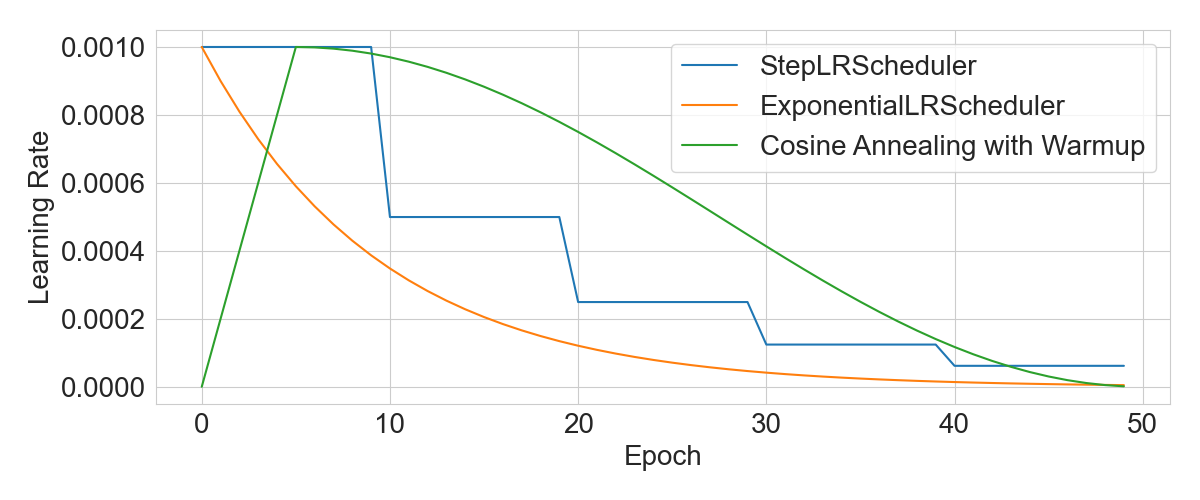
\includegraphics[height=70mm]{./figure/sec3/lr_scheduler.png}
    \caption{スケジューラによる学習率の変化}
    \label{sec3:fig:lr_scheduler}
\end{figure}

\subsubsection{正規化}
DNNの学習過程では学習の進行に伴って重みが変化するため、その度に各層への入力の分布が変わってしまう。これは内部共変量シフト(Internal Covariate Shift)と呼ばれ、ネットワークの学習を不安定にする原因となる。これに対し、バッチ正規化(Batch Normalization)\cite{ioffe2015batch}が有効である。バッチ正規化は、ミニバッチ学習を行う際にそのミニバッチ内における平均と標準偏差を計算し、特徴量を標準化する。バッチサイズを$N$、バッチ正規化への入力を$\{ \bm{x}_{i} \in \mathbb{R}^{D \times T} | 1 \le i \le N \}$とすると、出力$\bm{y}_{i} \in \mathbb{R}^{D \times T} ~ (1 \le i \le N)$は
\begin{align}
    \bm{\mu}_{\text{batch}}   & = \frac{1}{N} \sum_{i = 1}^{N} \bm{x}_{i}                                                  \\
    \sigma_{\text{batch}}^{2} & = \frac{1}{N} \sum_{i = 1}^{N} (\bm{x}_{i} - \bm{\mu}_{\text{batch}})^{2}                  \\
    \hat{\bm{x}_{i}}          & = \frac{\bm{x}_{i} - \bm{\mu}_{\text{batch}}}{\sqrt{\sigma_{\text{batch}}^{2} + \epsilon}} \\
    \bm{y}_{i}                & = \bm{\gamma} \hat{\bm{x}_{i}} + \bm{\beta}
\end{align}
で与えられる。ここで、$\bm{\mu}_{\text{batch}}, \bm{\sigma_{\text{batch}}} \in \mathbb{R}^{D}$はそれぞれミニバッチにおける平均ベクトルおよび分散ベクトル、$\bm{\gamma}, \bm{\beta} \in \mathbb{R}^{D}$は学習可能なベクトルである。バッチ正規化では入力を一度ミニバッチ内の平均と分散を用いて標準化した上で、学習可能なベクトル$\bm{\gamma}$の乗算と$\bm{\beta}$の加算により、表現力を向上させている。バッチ正規化は、畳み込み層や全結合層と合わせて用いられることが多い。

バッチ正規化はDNNの学習の安定化に貢献するが、一方で、バッチサイズが小さい場合はデータの分布を安定させることが難しくなるという課題がある。これに対し、ミニバッチ内の各データごとに平均と分散を求めて標準化する、レイヤー正規化(Layer Normalization)\cite{ba2016layer}がある。上記と同じ変数を用い、特にデータごとにチャンネル方向に平均と分散を求める場合、これは
\begin{align}
    \bm{\mu}_{\text{layer}}        & = \frac{1}{D} \sum_{d = 1}^{D} \bm{x}_{i, d}                                                     \\
    \bm{\sigma}_{\text{layer}}^{2} & = \frac{1}{D} \sum_{d = 1}^{D} (\bm{x}_{i, d} - \bm{\mu}_{layer})^{2}                            \\
    \hat{\bm{x}}_{i}               & = \frac{\bm{x}_{i} - \bm{\mu}_{\text{layer}}}{\sqrt{\bm{\sigma}_{\text{layer}}^{2}  + \epsilon}} \\
    \bm{y}_{i}                     & = \bm{\gamma} \hat{\bm{x}_{i}} + \bm{\beta}
\end{align}
で与えられる。ここで、$\bm{\mu}_{\text{layer}}, \bm{\sigma}_{\text{layer}} \in \mathbb{R}^{T}$が各データごとの平均ベクトルおよび分散ベクトルである。レイヤー正規化は、LSTMやGRU、Transformerといった一次元系列に対して適用されるニューラルネットワークと合わせて用いられることが多い。

上述したバッチ正規化およびレイヤー正規化はニューラルネットワーク内部で特徴量に対して適用する正規化であった。一方、ニューラルネットワークの重み自体を正規化する手法として、重み正規化(Weight Normalization)\cite{salimans2016weight}がある。これは、ある層の重みベクトルを$\bm{\theta}$とすると、
\begin{equation}
    \bm{\theta} = \frac{\bm{v}}{\| \bm{v} \|} g
\end{equation}
で与えられる。これは、重みベクトル$\bm{\theta}$を単位ベクトル$\bm{v} / \| \bm{v} \|$(ベクトルの向き)とスカラー$g$(ベクトルの大きさ)に分解することを意味する。重み正規化を適用した層については、重みの更新を$\bm{v}$と$g$それぞれで行う。重みの向きが大きさから分離されているため、損失関数の勾配に対して安定した重みの更新を行うことができるメリットがある。例えば、損失関数の勾配が大きい場合、通常は重みベクトルの向きおよび大きさを一括に動かして更新するが、重み正規化を適用しておけば、向きの更新の程度と大きさの更新の程度を分けて考えることができるため、学習が安定する可能性がある。重み正規化は、学習が不安定になりやすいGANのGeneratorやDiscriminatorに対して適用される場合がある。

\subsubsection{学習の安定化}
DNNの学習は勾配降下法によって行われるが、ここで勾配が大きくなりすぎると重みの更新幅が過剰に大きくなり、学習が不安定にある可能性がある。これに対して、Gradient Clippingが有効である。Gradient Clippingは、勾配のノルムが設定した閾値を超える場合に、勾配をスケーリングしてそのノルムを抑制する方法である。勾配の更新式は、勾配を$\bm{g}$、設定した閾値を$c$とすると、
\begin{equation}
    \bm{g} \gets \bm{g} \cdot \frac{c}{\max (\|\bm{g}\|_{2}, c)}
\end{equation}
で与えられる。ここで、$\|\bm{g}\|_{2}$は勾配のL2ノルムである。損失関数がスムーズに下がらない場合に、学習を安定させる一つの手段として有効である。

また、近年は数億単位のパラメータを持つ大規模なモデルも提案されており、こういった規模間のモデルを構築して学習する場合、それ相応のメモリが必要になる。これに対し、同一のマシンでもバッチサイズを小さくすることによって計算可能になると考えられるが、バッチサイズを小さくすることは各データのノイズの影響を強くする要因となり、学習が不安定になる可能性がある。このような状況では、Gradient Accumulationが有効である。Gradient Accumulationは、小さなバッチサイズで計算した勾配を複数回に渡って累積し、設定した回数ごとに重みの更新を行う手法である。各イテレーション$t$において得られる勾配を$\bm{g}_{t}$、累積される勾配を$\bm{g}_{\text{accum}}$とすると、$\bm{g}_{\text{accum}}$の更新は
\begin{equation}
    \bm{g}_{\text{accum}} \gets \bm{g}_{\text{accum}} + \bm{g}_{t}
\end{equation}
で与えられる。ここで、設定した累積回数を$k$、学習率を$\eta$とすると、$k$回に一回行う重み$\bm{\theta}$の更新は
\begin{equation}
    \bm{\theta} \gets \bm{\theta} - \eta \frac{\bm{g}_{\text{accum}}}{k}
\end{equation}
で与えられる。$k$回分の勾配を累積した分、重みを更新する際には$1 / k$にスケーリングすることで、実質的に$k$倍のバッチサイズにおける学習が可能になる。また、重み更新後は累積した勾配を0にリセットして、次の$k$回の累積に備える。

\subsubsection{自己教師あり学習}
近年、音声や動画を用いる分野では、自己教師あり学習(Self-Supervised Learning; SSL)を事前に行ったモデルを解きたい問題にFineTuningする、転移学習の有効性が確認されている。FineTuningするタスクは、下流タスク(Downstream Task)と呼ばれることが多い。ここで、自己教師あり学習とは、ラベルのないデータから特徴を学習するために、ラベルなしデータ自体から擬似的にラベルとなるものを作成して、それを元に教師あり学習を行う方法である。ラベルのないデータからそのデータの特徴を学習させるという点で、クラスタリングや次元削減などの教師なし学習に類似している。しかし、教師なし学習においては、ラベルなしデータから擬似ラベルを作成するという手順は踏まない。この点で、自己教師あり学習は教師あり学習に近い教師なし学習だと解釈できる。本研究においては、自己教師あり学習モデルのFineTuningを精度改善を目指したアプローチとして検討したため、本節では特に、本研究で検討対象とした事前学習済みモデルの行っている、Masked Predictionという自己教師あり学習の方法について述べる。

Masked Predictionでは、入力データの一部をマスクし、マスクされた領域の内容を予測するようにモデルを学習させる。穴埋め問題を解かせるイメージである。入力データを$\bm{X} \in \mathbb{R}^{T \times D}$、このうちマスクされるインデックスの部分集合を$\mathcal{M} \subset \{ 1, \ldots T \}$とする。この時、マスクされた入力$\bm{X}^{\text{masked}} \in \mathbb{R}^{T \times D}$は、
\begin{equation}
    \bm{X}^{\text{masked}}_{t} =
    \begin{cases}
        \bm{X}_{t} & \text{if $t \in \mathcal{M}$}    \\
        \bm{m}     & \text{if $t \notin \mathcal{M}$}
    \end{cases}
\end{equation}
で与えられる。ここで、$\bm{X}_{t}, \bm{X}^{\text{masked}}_{t} \in \mathbb{R}^{D}$はそれぞれ位置$t$における入力ベクトル、マスクされた入力ベクトルで、$\bm{m} \in \mathbb{R}^{D}$はマスクベクトルである。Masked Predictionではマスキングによって得られた$\bm{X}^{\text{masked}}$をモデルへの入力とし、$\bm{X}$を擬似ラベルとして学習を行う。ここで、音声の分野におけるHuBERT\cite{hsu2021hubert}や、動画音声の分野におけるAVHuBERT\cite{shi2022learning}では、扱うデータ自体が連続値となっているため、クラスタリングによる離散化を適用して擬似ラベルを作成する。ここで、クラスタ数を$C$とするクラスタリングによって得られた擬似ラベルを$\bm{X}^{\text{discretized}} \in \{0, 1\}^{T \times C}$とすると、モデルの予測値$\hat{\bm{X}} \in [0, 1]^{T \times C}$に対する損失は、
\begin{equation}
    L_{CE}(\bm{X}^{\text{discretized}}, \hat{\bm{X}}) =
    - \frac{1}{|\mathcal{M}|} \sum_{t \in \mathcal{M}} \sum_{c = 1}^{C} \bm{X}^{\text{discretized}}_{t, c} \log (\hat{\bm{X}}_{t, c})
\end{equation}
で与えられる。すなわち、マスクされた位置に限定したCross Entropy Lossである。この損失を最小化するようにモデルを学習させることで、特に音声や動画における文脈的な構造を学習させることが可能である。実際、HuBERTは音声からその発話内容を推定する音声認識、AVHuBERTは動画から発話内容を推定するVSRなどで、スクラッチで学習した場合と比較して高い精度を達成できることが示されている。近年ではこういったモデルを転移学習することが、下流タスクにおけるスタンダードになりつつある。

\clearpage

\section{動画音声合成モデルの検討}
\subsection{音声合成法}
提案手法の構築手順は3段階に分かれる。ネットワークの構造を図~\ref{sec4:fig:network}に示す。
一段階目では、動画を入力として、メルスペクトログラムとHuBERT離散特徴量、HuBERT中間特徴量を推定するネットワークAを学習する(図~\ref{sec4:fig:network}のA)。ここで、HuBERT離散特徴量はHuBERT Transformer層から得られる特徴量を k-means法によってクラスタリングすることで離散化した値、HuBERT中間特徴量はHuBERTにおける畳み込み層出力で、HuBERTの事前学習時にマスク対象となる値のことを指す。図~\ref{sec4:fig:hubert}にこれらの取得位置を示す。第一段階では、AVHuBERTを動画からの特徴抽出に利用した。これにより、動画の空間情報は完全に圧縮され、768次元の一次元系列となる。その後、事前学習済みの話者識別モデル\cite{wan2018generalized}によって音声波形から得られる256次元の話者Embeddingを、各フレームでチャンネル方向に結合する。これによって特徴量は1024次元に拡張され、全結合層によって再度768次元に圧縮する。その後、畳み込み層と全結合層からなるデコーダを通すことによって、話者Embeddingを結合した特徴量に対する変換を施した。これにより、特にメルスペクトログラムにおいて話者性が正しく反映されることを狙った。複数話者モデルであっても、入力である動画の見た目から話者性を判別できる可能性があったが、将来的な未知話者対応への拡張性も考慮して、本研究では補助特徴量として入力することとした。デコーダは残差結合を利用したブロック単位で構成され、各ブロックに2層の畳み込み層を設けた。各畳み込み層のチャンネル数は768、カーネルサイズは3であり、3ブロック積み重ねた。最後に全結合層を通し、所望の次元に変換することで予測対象を得た。ネットワークAの役割は、続くネットワークBの入力であるHuBERT中間特徴量を提供することである。これに対し、メルスペクトログラムとHuBERT離散特徴量の推定を同時に行った理由は、先行研究においてマルチタスク学習の有効性が確認されていることを考慮し、ネットワークAでもマルチタスク学習を採用しておこうと考えたからである。

二段階目では、一段階目に学習されたネットワークAの重みを固定した状態でHuBERT中間特徴量を推定し、それを入力としてメルスペクトログラムとHuBERT離散特徴量を推定する、HuBERT Transformer層を中心としたネットワークBの学習を行う(図~\ref{sec4:fig:network}のB)。HuBERT Transformer層出力はAVHuBERT出力と同じ768次元の特徴量となるため、これに対してネットワークAと同様に話者Embeddingを結合し、デコーダを通すことで予測値を得た。ネットワークBの役割は、音声波形への変換に必要となるメルスペクトログラムとHuBERT離散特徴量の予測である。HuBERT Transformer層の転移学習を検討した狙いについて、HuBERTは自己教師あり学習時、畳み込み層出力にマスクを適用し、Transformer層を通すことによってマスクされた部分を推定しようとする。これにより、音声の文脈を考慮するのに長けた学習済み重みが、特にTransformer層で獲得されると仮定した。これに基づき、本研究ではHuBERT Transformer層を動画音声合成にFine Tuningすることにより、動画を入力としたAVHuBERTを中心とするネットワークAにおける推定残差を、音声自体の文脈を考慮することによって軽減し、動画から直接推定しきれなかった部分を補うことでの精度改善を狙った。

\begin{figure}[bt]
    \centering
    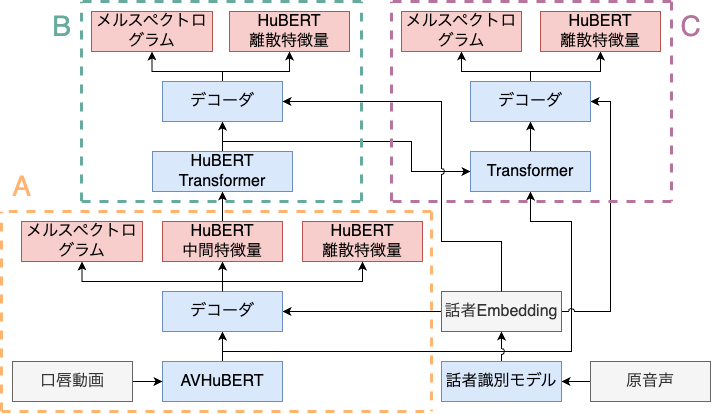
\includegraphics[height=90mm]{./figure/sec4/model/network.drawio.png}
    \caption{提案するネットワークの構造}
    \label{sec4:fig:network}
\end{figure}

\begin{figure}[bt]
    \centering
    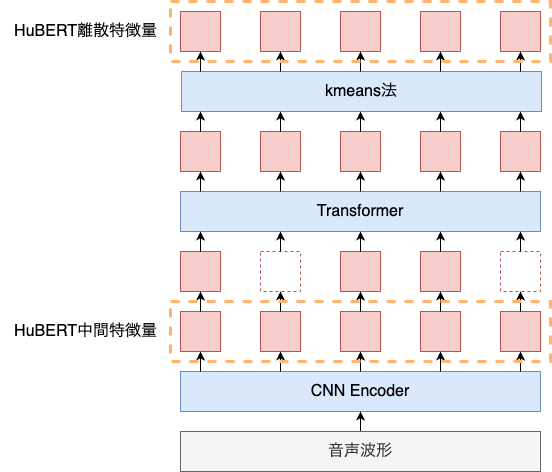
\includegraphics[height=90mm]{./figure/sec4/model/hubert.png}
    \caption{HuBERT中間特徴量とHuBERT離散特徴量の取得位置}
    \label{sec4:fig:hubert}
\end{figure}

三段階目では、二段階目までに学習されたネットワークAとネットワークBの重みを固定した状態で、AVHuBERTから得られる特徴量と、HuBERT Transformer層から得られる特徴量の二つを結合し、それらを入力として再びメルスペクトログラムとHuBERT離散特徴量の予測を行うネットワークCを学習した(図~\ref{sec4:fig:network}のC)。ネットワークCでは、はじめに前述した二つの特徴量をチャンネル方向に結合することで、1536次元の入力特徴量を得る。これに対して全結合層を施すことで再度768次元に圧縮し、4層のTransformer層を通すことで系列全体を考慮した特徴抽出を改めて行った。その後、ネットワークA,Bと同様に話者Embeddingを結合し、デコーダを通すことによって予測値を得た。ここで、ネットワークCのTransformer層におけるパラメータについては、AVHuBERTやHuBERTと同様にチャンネル数を768、ヘッド数は12とした。ネットワークCの役割は、ネットワークBと同様に音声波形への変換に必要な特徴量の予測である。ここでの狙いについて、まず、AVHuBERTから得られる特徴量とHuBERT Transformer層から得られる特徴量は、どちらもデコーダへの入力となる点で同じである。一方、AVHuBERTは動画を入力、HuBERT Transformer層はHuBERT中間特徴量を入力とするため、これら特徴量の元となる入力は異なっている。ここでは、概ね同じ予測対象のために利用される二つの特徴量(ネットワークAではHuBERT中間特徴量の予測も行っているため、全く同じではない)が、入力の違いに依存して内部のSelf Attentionにより注意される部分が変化し、何らかの異なった情報を持っている可能性があると仮定した。よって、両方の特徴量を考慮し、単一特徴量への依存を解消することで、汎化性能向上による予測精度の改善を狙った。

以上が提案手法の全体像であるが、今回ベースラインとする先行研究\cite{choi2023intelligible}に基づいたマルチタスク学習手法は、本研究におけるネットワークAで、HuBERT中間特徴量を推定しないものに当たる。

以上のモデルにより、動画からメルスペクトログラムとHuBERT離散特徴量が推定可能となる。その後、先行研究\cite{choi2023intelligible}に基づくMulti-input Vocoderを用い、メルスペクトログラムとHuBERT離散特徴量を入力として音声波形に変換することで、最終的な合成音声を得た。Multi-input VocoderはHiFi-GAN\cite{kong2020hifi}をベースとしたモデルであり、音声波形を生成するGeneratorと、Multi-Period Discriminator(MPD)およびMulti-Scale Discriminator(MSD)という二つのDiscriminatorによって構成される。

Generatorの構造を図~\ref{sec4:fig:multi-input_vocoder}に示す。左の特徴量予測モデルは、動画からメルスペクトログラムとHuBERT離散特徴量を予測する、本研究において主な検討対象となる部分を表す。Generatorの内部構造について、まず、前処理層はメルスペクトログラムとHuBERT離散特徴量を入力として受け取り、その後のレイヤーに入力するための形状に変換する役割を持つ。メルスペクトログラムに対しては、時間方向に隣接した2フレームを次元方向に縦積みすることによって、100 Hz・80次元の特徴量から50 Hz・160次元の特徴量に変換した後、全結合層によって128次元の特徴量に変換する。一方、HuBERT離散特徴量は50 Hzのインデックス系列であり、インデックスから128次元のベクトルへと変換する。その後、これらをチャンネル方向に結合することで50 Hz・256次元の特徴量を構成し、これをその後のレイヤーへの入力とする。この特徴量は、転置畳み込み層と複数種類の畳み込み層から構成されるブロックを通過していく。各ブロックについて、まず、転置畳み込み層は特徴量を時間方向にアップサンプリングする役割を果たす。実際、本研究では50 Hzの入力特徴量から16 kHzの音声波形まで、時間方向に320倍のアップサンプリングを行う必要がある。Generatorでは、これを複数のブロックを通して段階的に行っている。また、各ブロックの転置畳み込み層に積まれた複数種類の畳み込み層は、そのカーネルサイズとダイレーションが全て異なっている。複数の時間的な受容野を持つ畳み込み層からの出力をすべて加算することで、アップサンプリング後の特徴量からの特徴抽出を行う仕組みとなっている。表~\ref{sec4:tab:multi-input_vocoder_parameter}に、Generatorの各ブロックにおけるパラメータとブロックごとの出力特徴量の形状を示す。カラム名の右にある括弧がきが数値の意味を表しており、Kはカーネルサイズ、Sはストライド、Dはダイレーション、Cは次元(チャンネル数)、Tは系列長である。畳み込み層についてはカーネルサイズとダイレーションを集合として表記しているが、実際はこれらの直積の元、すなわち(3, 1)や(3, 3)、(3, 5)をパラメータとする畳み込み層が存在することを表す。すなわち、転置畳み込み層一層に対し、その後の特徴量抽出は15種類の異なるカーネルサイズ、ダイレーションを設定した畳み込み層によって行われる。
\begin{figure}[bt]
    \centering
    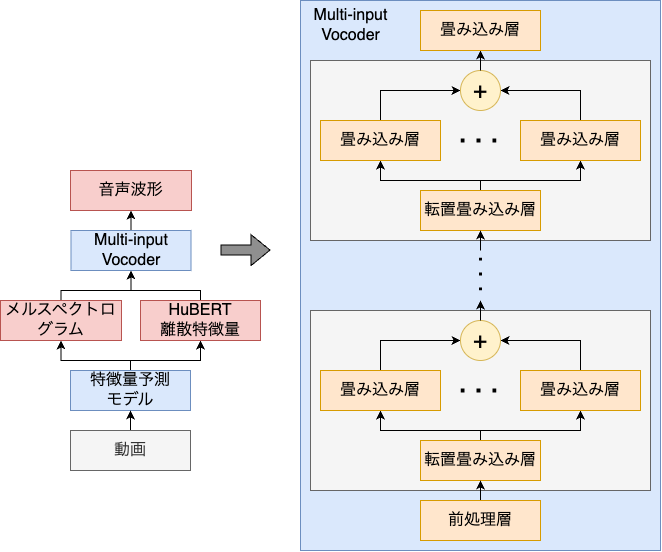
\includegraphics[height=120mm]{./figure/sec4/model/multi-input_vocoder.png}
    \caption{Multi-input Vocoderの構造}
    \label{sec4:fig:multi-input_vocoder}
\end{figure}
\begin{table*}[bt]
    \centering
    \caption{Generatorの各ブロックにおけるパラメータ}
    \label{sec4:tab:multi-input_vocoder_parameter}
    \begin{center}
        \renewcommand{\arraystretch}{0.9} % 行の高さ調整
        \setlength{\tabcolsep}{8pt}      % 列の幅調整
        \scalebox{1.0}{
            \begin{tabular}{|c|c|c|c|}
                \hline
                  & \multicolumn{1}{c|}{転置畳み込み層 (K, S)} & \multicolumn{1}{c|}{畳み込み層 (K, D)}     & \multicolumn{1}{c|}{出力特徴量の形状 (C, T)} \\
                \hline
                1 & (11, 5)                             & ($\{3, 5, 7, 9, 11\}$, $\{1, 3, 5\}$) & (1024, 250)                          \\
                2 & (8, 4)                              & ($\{3, 5, 7, 9, 11\}$, $\{1, 3, 5\}$) & (512, 1000)                          \\
                3 & (4, 2)                              & ($\{3, 5, 7, 9, 11\}$, $\{1, 3, 5\}$) & (256, 2000)                          \\
                4 & (4, 2)                              & ($\{3, 5, 7, 9, 11\}$, $\{1, 3, 5\}$) & (128, 4000)                          \\
                5 & (4, 2)                              & ($\{3, 5, 7, 9, 11\}$, $\{1, 3, 5\}$) & (64, 8000)                           \\
                6 & (4, 2)                              & ($\{3, 5, 7, 9, 11\}$, $\{1, 3, 5\}$) & (32, 16000)                          \\
                \hline
            \end{tabular}
        }
    \end{center}
\end{table*}

Generatorの学習時に用いられるのが、MPDおよびMSDという二つのDiscriminatorである。これらの概要を図~\ref{sec4:fig:multi-input_vocoder_mpd_msd}に示す。MPDでは、一次元の音声波形を指定した周期をもとにReshapeすることで二次元に変換し、これに対して二次元畳み込みを適用することで、入力された音声波形の原音声らしさを判定するDiscriminatorである。異なる周期を設定したDiscriminatorを複数利用することで、時間的な特徴を考慮できるように構成されている。一方、MSDでは、音声波形に対してAverage Poolingを適用することでダウンサンプリングし、これに一次元畳み込みを適用することで入力された音声波形の原音声らしさを判定するDiscriminatorである。MSDはAverage Poolingによって系列長を抑えつつ、時間方向の連続的な特徴を考慮する狙いがある。これら二つのDiscriminatorについては、HiFi-GANと同様のパラメータで用いた。
\begin{figure}[bt]
    \centering
    \begin{subfigure}{0.45\textwidth}
        \centering
        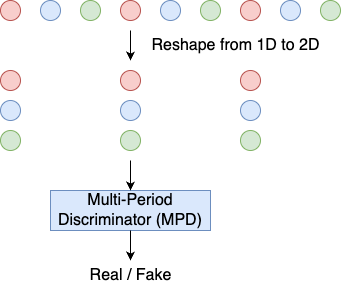
\includegraphics[width=\linewidth]{./figure/sec4/model/mpd.png}
        \caption{Multi-Period Discriminator(MPD)}
        \label{sec4:fig:multi-input_vocoder_mpd}
    \end{subfigure}
    \hfill
    \begin{subfigure}{0.45\textwidth}
        \centering
        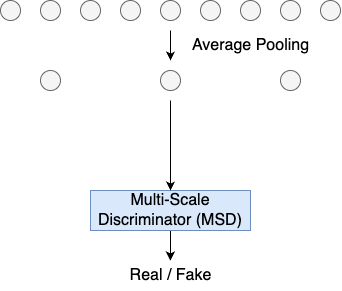
\includegraphics[width=\linewidth]{./figure/sec4/model/msd.png}
        \caption{Multi-Scale Discriminator(MSD)}
        \label{sec4:fig:multi-input_vocoder_msd}
    \end{subfigure}
    \caption{Multi-Period Discriminator(MPD)とMulti-Scale Discriminator(MSD)の概要}
    \label{sec4:fig:multi-input_vocoder_mpd_msd}
\end{figure}

\subsection{実験方法}
\subsubsection{利用したデータセット}
動画音声データセットには、男女二人ずつから収録した合計4人分のデータセット\cite{taguchi,esaki}を用いた。これはATR音素バランス文\cite{atr}から構成され、全話者共通でAからHセットを学習データ、Iセットを検証データ、Jセットをテストデータとして利用した。各分割ごとの文章数を表~\ref{sec4:tab:dataset_info}に示す。

Multi-input Vocoderの学習に利用する音声データセットには、Hi-Fi-Captain(日本語話者二名分)\cite{okamoto2023hi}とJVS(parallel100とnonpara30)\cite{takamichi2019jvs}を利用した。Hi-Fi-Captainはtrain-parallelおよびtrain-non-parallelを学習データ、valを検証データ、evalをテストデータとして分割した。各分割ごとの文章数を表~\ref{sec4:tab:dataset_info}に示す。JVSには話者に対して1から100まで番号が割り振られており、本実験では1から80番の話者を学習データ、81番から90番の話者を検証データ、91番から100番までの話者をテストデータとした。各分割ごとの文章数を表~\ref{sec4:tab:dataset_info}に示す。また、JVSには読み上げ音声のparallel100およびnonpara30と、裏声のfalset10、囁き声のwhisper10が含まれる。本研究では、parallel100とnonpara30のみを利用した。

\begin{table*}[bt]
    \centering
    \caption{利用したデータセットの文章数}
    \label{sec4:tab:dataset_info}
    \begin{center}
        \renewcommand{\arraystretch}{0.9} % 行の高さ調整
        \setlength{\tabcolsep}{8pt}      % 列の幅調整
        \scalebox{1.0}{
            \begin{tabular}{|l|r|r|r|}
                \hline
                              & \multicolumn{1}{c|}{学習} & \multicolumn{1}{c|}{検証} & \multicolumn{1}{c|}{テスト} \\
                \hline
                動画音声データセット    & 1598                    & 200                     & 212                      \\
                Hi-Fi-Captain & 37714                   & 200                     & 200                      \\
                JVS           & 10398                   & 1299                    & 1300                     \\
                \hline
            \end{tabular}
        }
    \end{center}
\end{table*}

\subsubsection{データの前処理}
動画データは60 FPSで収録されたものをffmpegにより25 FPSに変換して用いた。その後、手法\cite{bulat2017far}により動画に対してランドマーク検出を適用した。このランドマークを利用することで口元のみを切り取り、画像サイズを(96, 96)にリサイズした。モデル入力時は動画をグレースケールに変換し、各フレームに対する正規化および標準化を適用した。正規化では、グレースケールが0から255までの値を取るため、最大値の255で割り、標準化では、AVHuBERTのプログラムで利用されていた平均値0.421と、標準偏差0.165をそのまま利用して、平均値を引いた後に標準偏差で割った。全体として、今回は事前学習済みのAVHuBERTの転移学習を行うため、そこでの前処理に合わせている。学習時は、ランダムクロップ、左右反転、Time Masking(一時停止)をデータ拡張として適用した。ランダムクロップは、(96, 96)で与えられる画像から(88, 88)をランダムに切り取る処理である。検証およびテスト時は、必ず画像中央を切り取るよう実装した。左右反転は、50\%の確率で左右が反転されるよう実装した。Time Maskingは、連続する画像の時間平均値を利用することによって、一時停止させるような効果を与えるデータ拡張手法である。動画1秒あたり0から0.5秒の間でランダムに停止区間を定め、その区間における動画の時間方向平均値を計算し、区間内のすべてのフレームをこの平均値で置換した。

音声データは16 kHzにダウンサンプリングして用いた。それから、窓長25 msのハニング窓を用いて、シフト幅10 msでSTFTを適用することでフレームレート100 Hzのスペクトログラムに変換した。さらに、パワースペクトログラムに対して80次のメルフィルタバンクを適用し、メルスペクトログラムを得た上で対数スケールに変換した。
また、Multi-input Vocoderの学習に利用したHi-Fi-CaptainとJVSについては、無音区間のトリミング(-40 dBFS未満かつ500 ms継続する区間を100 msまでカット)を適用した。なぜなら、Multi-input Vocoderの学習時は、全体から1秒分をランダムサンプリングするように実装しており、元データに存在する無音区間を除去することによって、学習の安定化および得られる音声の品質改善に繋がったからである。
また、話者Embeddingの取得には事前学習済みの話者識別モデル\cite{wan2018generalized}を利用した。動画音声データセット、Hi-Fi-Captain、JVSともに、各話者学習データの中から100文章をランダムサンプリングし、各発話に対して得られたベクトルの平均値を用いた。この値を学習・検証・テストで一貫して用いるため、学習外の検証データやテストデータには非依存な値となっている。モデルに入力する際には、ベクトルの大きさで割って正規化した。

HuBERTは、HuggingFaceに公開されているReazonSpeechというデータセットによって学習されたモデル\cite{rinna-japanese-hubert-base,sawada2024release}を利用した。ReazonSpeechは約19000時間の日本語音声からなるデータセットであり、日本語音声のコンテキストを大量のデータから学習したモデルである。今回用いるデータセットが日本語であることから、本研究の検討対象としては日本語音声に関する事前知識を豊富に有するモデルが適していると考え、このモデルを選択した。本研究で用いるHuBERT中間特徴量およびHuBERT離散特徴量について、HuBERT中間特徴量は、音声波形に対して畳み込み層を適用した出力で、HuBERTの事前学習時にはマスクの対象となる特徴量を利用した。一方、HuBERT離散特徴量は、HuBERT Transformer層の8層目出力に、k-means法によるクラスタリングを適用することで得た。あえて8層目出力を選択した理由は、HuBERTのレイヤーごとの特徴量について、音素のOne-hotベクトルおよび単語のOne-hotベクトルとの相関を、Canonical Correlation Analysis(CCA)によって調べた先行研究\cite{pasad2023comparative}より、8層目出力がそのどちらとも相関が高く言語的な情報に近いと判断したからである。クラスタ数については決め打ちとなるが、今回は離散化した結果が言語的な情報を持つことを狙い、比較的少ない100とした。k-means法の学習には動画音声データセットにおける学習用データ全てを利用し、これを用いて動画音声データ、Hi-Fi-Captain、JVSに対するクラスタリングを実施した。

\subsubsection{学習方法}
一段階目について、損失関数はメルスペクトログラムのMAE Loss $L_{mel}$ とHuBERT離散特徴量のCross Entropy Loss $L_{ssl^{d}}$ 、HuBERT中間特徴量のMAE Loss $L_{ssl^{i}}$ の重み付け和とした。それぞれの重み係数を$\lambda_{mel}, \lambda_{ssl^{d}}, \lambda_{ssl^{i}}$とすると、
\begin{equation}
    \label{sec4:eq:loss}
    L = \lambda_{mel} * L_{mel} + \lambda_{ssl^{d}} * L_{ssl^{d}} + \lambda_{ssl^{i}} * L_{ssl^{i}}
\end{equation}
となる。最適化手法にはAdamW\cite{loshchilov2017decoupled}を利用し、$\beta_{1} = 0.9$、$\beta_{2} = 0.98$、$\lambda = 0.01$とした。学習率に対するスケジューラには、Cosine Annealing with Warmupを利用した。開始時の学習率は\num{1.0e-6}として、最大エポック数の10\%に至るまでは学習率を\num{1.0e-3}まで線形に増加させ、その後のエポックではcosine関数に基づいて\num{10.e-6}まで減少させた。バッチサイズはメモリの都合上4としたが、学習の安定化のため、Gradient Accumulationによって各イテレーションにおける勾配を累積させ、8イテレーションに一回重みを更新するようにした。モデルに入力する動画の秒数は10秒を上限とし、それを超える場合はランダムにトリミング、それに満たない場合はゼロパディングした。ゼロパディングした部分は損失の計算からは除外した。勾配のノルムは3.0を上限としてクリッピングすることで、過度に大きくなることを防止した。最大エポック数は50とし、10エポック連続して検証データに対する損失が小さくならない場合には、学習を中断するようにした(Early Stopping)。また、学習終了時には検証データに対する損失が最も小さかったエポックにおけるチェックポイントを保存し、これをテストデータに対する評価に用いた。

第二段階について、損失関数はメルスペクトログラムのMAE LossとHuBERT離散特徴量のCross Entropy Lossの重み付け和とした。これは式~\eqref{sec4:eq:loss}において、$\lambda_{ssl^{i}} = 0.0$と固定した場合に相当する。最適化手法にはAdamWを利用し、$\beta_{1} = 0.9$、$\beta_{2} = 0.98$、$\lambda = 0.01$とした。学習率に対するスケジューラには、Cosine Annealing with Warmupを利用した。開始時の学習率は\num{1.0e-6}として、最大エポック数の10\%に至るまでは学習率を\num{5.0e-4}まで線形に増加させ、その後のエポックではcosine関数に基づいて\num{10.e-6}まで減少させた。学習率の最大値は第一段階の$1/2$となっているが、これは値を半減させることによって学習を安定させることができたためである。その他のパラメータは、第一段階における値と同じである。

第三段階について、Cosine Annealing with Warmupにおける最大学習率のみ\num{1.0e-3}としたが、それ以外は第二段階と同様である。

Multi-input Vocoderの学習では、Hi-Fi-CaptainとJVSを用いた。はじめにHi-Fi-Captainのみを用いて学習させ、その後学習済みモデルをJVSによって再学習した。損失関数はHiFi-GANと同様である。二つのデータセットを用いた理由について、Hi-Fi-Captainは男女一人ずつの文章数が豊富なデータセットであるため、高品質なモデルを構築可能であった。しかし、学習できる話者数が少ない分、学習外話者に対する合成音声の品質が低かった。そのため、一人当たりの文章数は100文章程度と少ないながらも、100人分の話者からなるJVSを利用して再学習することによって、学習外話者に対する合成音声の品質を向上させた。最適化手法にはAdamWを利用し、$\beta_{1} = 0.8$、$\beta_{2} = 0.99$、$\lambda = \num{1.0e-5}$とした。学習率は\num{2.0e-4}から開始し、1エポック経過するごとに0.99かけて徐々に減衰させた。バッチサイズは16とし、ここではGradient Accumulationは利用しなかった。モデルへの入力は1秒を上限とし、それを超える場合はランダムにトリミング、それに満たない場合はゼロパディングした。勾配のノルムは3.0を上限としてクリッピングすることで、過度に大きくなることを防止した。最大エポック数は30とし、ここではEarly Stoppingは適用しなかった。また、学習終了時には検証データに対する損失(メルスペクトログラムに対するL1 Loss)が最も小さかったエポックにおけるチェックポイントを保存し、これをテストデータに対する評価に用いた。また、Multi-input Vocoderの提案された先行研究\cite{choi2023intelligible}においては、学習時にあえてメルスペクトログラムにノイズをかけることによって、合成音声に対する汎化性能を向上させる学習方法が提案されている。本研究では、動画から推定されるメルスペクトログラムとHuBERT離散特徴量の推定精度向上に焦点を当てたため、Multi-input Vocoderの学習は原音声から計算される特徴量そのもので行い、ボコーダ自体の汎化性能向上による精度改善は追求しなかった。

実装に用いた深層学習ライブラリはPyTorchおよびPyTorch Lightningである。GPUにはNVIDIA RTX A4000を利用し、計算の高速化のためAutomatic Mixed Precisionを適用した。

\subsubsection{客観評価}
合成音声の客観評価には、二種類の指標を用いた。
一つ目は、音声認識の結果から算出した単語誤り率(Word Error Rate; WER)である。WERの計算方法について、まず、正解文字列$s_{1}$と音声認識モデルによる予測文字列$s_{2}$に対し、レーベンシュタイン距離によってその差分を測る。レーベンシュタイン距離は、二つの文字列を一致させるために必要なトークンの挿入数$I$、削除数$D$、置換数$R$の和の最小値として定義される。WERは、レーベンシュタイン距離を測ることによって得られた$I, D, R$を利用し、
\begin{equation}
    \text{WER}(s_{1}, s_{2}) = \frac{I + D + R}{|s_{1}|}
\end{equation}
で与えられる。ここで、$|s_{1}|$は正解文字列$s_{1}$のトークン数を表す。実際には、音声認識モデルにWhisper\cite{radford2023robust}を利用し、出力される漢字仮名交じり文に対してMeCabを用いて分かち書きを行った上で、jiwerというライブラリを用いて算出した。WhisperはLargeモデルを利用し、MeCabの辞書にはunidicを利用した。WERの値は0\%から100\%であり、この値が低いほど音声認識の誤りが少ないため、より聞き取りやすい音声であると判断した。

二つ目は、話者Embeddingから計算したコサイン類似度である。モデルへの入力値を計算するのに用いた話者識別モデルを同様に利用し、サンプルごとに評価対象音声の話者Embeddingと原音声の話者Embeddingのペアでコサイン類似度を計算した。今回構築するモデルは4人の話者に対応するモデルとなるため、原音声に似た声質の合成音声が得られているかをこの指標で評価した。値は0から1であり、高いほど原音声と類似した合成音声だと判断できる。

\subsubsection{主観評価}
\label{sec4:sec:sbj_explanation}
合成音声の主観評価では、音声の明瞭性と類似性の二点を評価した。今回はクラウドワークスというクラウドソーシングサービスおよび、自作の実験用Webサイトを利用してオンラインで実験を実施した。被験者の条件は、日本語母語話者であること、聴覚に異常がないこと、イヤホンあるいはヘッドホンを用いて静かな環境で実験を実施可能であることとした。被験者の方に行っていただいた項目は、以下の五つである。
\begin{enumerate}
    \item アンケート
    \item 練習試行(明瞭性)
    \item 本番試行(明瞭性)
    \item 練習試行(類似性)
    \item 本番試行(類似性)
\end{enumerate}

一つ目のアンケートでは、被験者についての基本的な統計を取ることを目的として、性別・年齢・実験に利用した音響機器について回答してもらった。性別は、男性、女性、無回答の三つからの選択式とした。年齢は被験者の方に直接数値を入力してもらう形式とした。実験に使用した音響機器は、イヤホン、ヘッドホンの二つからの選択式とした。

二つ目の練習試行(明瞭性)および三つ目の本番試行(明瞭性)では、音声の明瞭性の評価を実施した。初めに練習試行を行っていただくことで実験内容を把握してもらい、その後本番施行を行っていただく流れとした。ここで、練習施行は何度でも実施可能とし、本番試行は一回のみ実施可能とした。
評価項目について、明瞭性は「話者の意図した発話内容を、一回の発話でどの程度聞き取ることができたか」を評価するものとした。実際の評価プロセスは以下の二段階で構成した。
\begin{enumerate}
    \item 音声サンプルのみを一回再生し、発話内容を聞き取ってもらう。
    \item 本来の発話内容を確認してもらい、聴取者が想定していた発話内容と本来の発話内容を照らし合わせ、音声の聞き取りやすさを5段階評価してもらう。
\end{enumerate}
5段階評価の回答項目は以下のようにした。
\begin{enumerate}
    \item 全く聞き取れなかった
    \item ほとんど聞き取れなかった
    \item ある程度聞き取れた
    \item ほとんど聞き取れた
    \item 完全に聞き取れた
\end{enumerate}

実験に利用した音声サンプルについて、練習試行では検証データ、本番試行ではテストデータを用いた。被験者ごとの評価サンプルの割り当て方法をアルゴリズム\ref{sec4:algo:sample-assignment}に示す。$\text{sentences}$は文章のリスト、$\text{method\_names}$が手法名のリスト、$\text{speaker\_names}$が話者名のリスト、$\text{num\_total\_respondents}$が被験者総数である。各被験者について、まず$\text{sentences}$と$\text{method\_names}$をランダムにシャッフルし、それからランダムサンプリングした$\text{speaker\_name}$を合わせて、一つのサンプルを決定するようになっている。この選択方法では、二つのことに注意した。一つ目は、各被験者がユニークな53文章を評価することである。評価の際に本来の発話内容を知ることになるため、それを知った上で同じ発話内容のサンプルが出現した場合、音声自体の明瞭性に関わらず発話内容がわかってしまう可能性があると考え、これを避けるようにした。二つ目は、各手法がなるべく均等な回数出現することである。今回は手法の比較が実験の目的となるため、各被験者がすべての手法を評価することが望ましいと判断した。また、評価に際し音声サンプルを一回だけ聞いてもらうようにした理由は、代用音声をコミュニケーションツールとして利用する場面を想定したとき、会話において何度も聞き返されることはストレスになると考えられるため、一回の発話で意図した発話内容をどの程度聞き取ってもらえるかをその手法の聞き取りやすさとして評価するべきだと考えたからである。
\begin{algorithm}
    \caption{Sample Assignment Algorithm}
    \label{sec4:algo:sample-assignment}
    \begin{algorithmic}[1]
        \Require \text{sentences}: List of sentences
        \Require \text{method\_names}: List of method names
        \Require \text{speaker\_names}: List of speaker names
        \Require \text{num\_total\_respondents}: Total number of respondents
        \State Initialize \text{all\_assignments} $\gets$ []
        \For{\text{respondent\_id} $\gets 1$ to \text{num\_total\_respondents}}
        \State Initialize \text{assignments} $\gets$ []
        \State Randomly shuffle \text{sentences}
        \State Randomly shuffle \text{method\_names}
        \For{$i \gets 0$ to $\text{len(sentences)} - 1$}
        \State \text{sentence} $\gets \text{sentences}[i]$
        \State \text{method\_name} $\gets \text{method\_names}[i \bmod \text{len(method\_names)}]$
        \State \text{speaker\_name} $\gets$ Randomly select from \text{speaker\_names}
        \State Append $(\text{respondent\_id}, \text{sentence}, \text{method\_name}, \text{speaker\_name})$ to \text{assignments}
        \EndFor
        \State \text{all\_assignments} $\gets \text{all\_assignments} \cup \text{assignments}$
        \EndFor
        \State \Return \text{all\_assignments}
    \end{algorithmic}
\end{algorithm}

四つ目の練習試行(類似性)および五つ目の本番試行(類似性)では、評価対象の音声と同一話者の原音声の類似性の評価を実施した。ここでも初めに練習試行を行っていただくことで実験内容を把握してもらい、その後本番施行を行っていただく流れとした。ここで、練習施行は何度でも実施可能とし、本番試行は一回のみ実施可能とした。
評価項目について、類似性は「評価対象の音声が同一話者の原音声とどれくらい似ているか」を評価するものとした。実際の評価プロセスは以下の二段階で構成した。
\begin{enumerate}
    \item 評価対象の音声と原音声を聞き比べてもらう。
    \item 評価対象の音声が原音声にどれくらい似ていたかを五段階評価してもらう。
\end{enumerate}
5段階評価の回答項目は以下のようにした。
\begin{enumerate}
    \item 全く似ていなかった
    \item あまり似ていなかった
    \item やや似ていた
    \item かなり似ていた
    \item 同じ話者に聞こえた
\end{enumerate}
実験に利用した音声サンプルおよび、被験者ごとの評価サンプルの割り当て方法は明瞭性の評価実験と同様にした。ただし、類似性評価においては、評価対象となる音声に対して同一話者の原音声をランダムに選択し、評価対象となる音声とペアで提示できるようにした。また、明瞭性評価では音声サンプルを一回だけ聞いて評価してもらうようにしたが、類似性評価では何度でも聞けるようにした。聞き取りやすさのようにコミュニケーションを想定した評価というより、単に原音声とどの程度似ているかを評価したいと考えたからである。さらに、明瞭性評価では評価時に発話内容を提示したが、類似性評価は発話内容に依存しないため、提示しなかった。類似性評価は発話内容に依存しないと考えらえるからである。加えて、類似性評価は明瞭性評価を完了した後にしか実施できないようにした。類似性評価と明瞭性評価に用いるサンプルは同一の発話内容のパターンであり、特に類似性評価では原音声を聴取できることから、本来の発話内容を完全に把握できると予想される。その上で明瞭性評価を行った場合、音声自体の明瞭性に関わらず発話内容がわかってしまう可能性があると考えられ、望ましくない。一方、類似性評価は発話内容に依存しない評価であるため、発話内容を知っていることが評価に影響を与えないと考えられる。よって、今回は明瞭性評価の後に類似性評価を行うことにした。

また、オンラインでの評価は効率よく数多くの方に評価していただけるという点でメリットがあるが、オフラインでの評価と比較して実験環境を制御することが難しく、評価品質が低下する恐れがある。これに対して、本実験では先行研究\cite{kirkland2023stuck}を参考に、評価サンプル中にダミー音声を混入させることで対策を講じた。ダミー音声は本研究で得られた合成音声とは無関係に、gTTSというライブラリを用いて生成したサンプルである。具体例として、明瞭性評価では
\begin{quote}
    これはダミー音声です。明瞭性は「3: ある程度聞き取れた」を選択してください。
\end{quote}
のような発話内容の音声を、類似性評価では
\begin{quote}
    これはダミー音声です。類似性は「1: 全く同じ話者には聞こえなかった」を選択してください。
\end{quote}
のような発話内容の音声を提示した。この時、その音声自体の明瞭性や類似性とは無関係に、必ずこの音声によって指定された評価値を選択するよう説明を与えた。本番試行においてダミー音声で指定された評価値を誤って選んだ場合は、すべての回答を無効にする旨を被験者に伝えた。実際、実験終了後にはそのようにデータを処理した。

被験者数は75人とし、謝礼は実験一回あたり40分程度要すると予想し、650円とした。

\subsection{結果}
\subsubsection{客観評価1: ベースラインと提案手法の比較}
\label{sec4:sec:obj_1}
本節では、ベースラインと提案手法の比較を行う。比較手法は、以下の五つである。
\begin{enumerate}
    \item ベースライン
    \item ネットワークA
    \item ネットワークB(Not-Pretrained)
    \item ネットワークC(Not-Pretrained)
    \item ネットワークB(Pretrained)
    \item ネットワークC(Pretrained)
\end{enumerate}
ベースラインは、提案手法(図\ref{sec4:fig:network})におけるネットワークAで、メルスペクトログラムとHuBERT離散特徴量を予測するマルチタスク学習手法である。ネットワークAは提案手法において、ネットワークBおよびCに入力を与える役割を果たすネットワークである。提案手法自体ではないが、その構成要素とはなっているため、ここでも客観評価指標を確認することとした。ネットワークB(Not-Pretrained)は、HuBERT Transformer層で事前学習済み重みを読み込まなかった場合のネットワークBである。これに関連して、ネットワークC(Not-Pretrained)はネットワークB(Not-Pretrained)を利用したネットワークCである。これらに対し、ネットワークB(Pretrained)およびネットワークC(Pretrained)は、ネットワークBの学習時にHuBERT Transformer層で事前学習済み重みを読み込んだ点のみ異なる。

まず、損失関数~\eqref{sec4:eq:loss}の重み係数$\lambda_{ssl^{d}}$を変化させた時の、客観評価指標の全テストデータに渡る平均値を表~\ref{sec4:tab:obj_weights}に示す。各手法ごとに$\lambda_{ssl^{d}}$を0.0001から1.0まで、10倍刻みで5段階検討するグリッドサーチを行い、各手法の客観評価指標ごとに、最も優れた値を下線で示している。ここで、提案手法ではネットワークAを学習し、その後Aを固定してBを学習し、最後にAとBを固定してCを学習するように実装している。これに対し、$\lambda_{ssl}^{d}$のグリッドサーチでは、この一連の流れに対して一つの値を検討した。例えば、ネットワークB(Not-Pretrained)で$\lambda_{ssl^{d}}$が0.0001の場合、ネットワークAには$\lambda_{ssl^{d}}$が0.0001の場合を用いている。ネットワークC(Not-Pretrained)で$\lambda_{ssl^{d}}$が0.0001の場合、ネットワークA、Bともに$\lambda_{ssl^{d}}$が0.0001の場合を用いている。また、この後手法ごとの比較を行う際には、各手法ごとにグリッドサーチで得られた最適な場合同士を比較するため、最適だと判断した場合を太字で示している。

\begin{table*}[bt]
    \centering
    \caption{損失関数の重み係数$\lambda_{ssl^{d}}$による客観評価指標の比較}
    \label{sec4:tab:obj_weights}
    \begin{center}
        \renewcommand{\arraystretch}{1.0} % 行の高さ調整
        \setlength{\tabcolsep}{8pt}      % 列の幅調整
        \scalebox{1.0}{
            \begin{tabular}{|c|l|rr|}
                \hline
                \multicolumn{1}{|c|}{手法}         & \multicolumn{1}{c|}{$\lambda_{ssl^{d}}$} & \multicolumn{1}{c}{WER [\%]} & \multicolumn{1}{c|}{話者類似度} \\
                \hline
                ベースライン                           & 0.0001                                   & 57.3                         & 0.833                      \\
                \textbf{ベースライン}                  & \textbf{0.001}                           & \underline{\textbf{54.6}}    & \textbf{0.836}             \\
                ベースライン                           & 0.01                                     & 56.2                         & \underline{0.837}          \\
                ベースライン                           & 0.1                                      & 58.2                         & 0.784                      \\
                ベースライン                           & 1                                        & 59.0                         & 0.685                      \\
                \hline
                ネットワークA                          & 0.0001                                   & 55.4                         & 0.841                      \\
                ネットワークA                          & 0.001                                    & 55.1                         & 0.842                      \\
                ネットワークA                          & 0.01                                     & \underline{53.4}             & \underline{0.843}          \\
                ネットワークA                          & 0.1                                      & 54.6                         & 0.809                      \\
                ネットワークA                          & 1                                        & 58.7                         & 0.698                      \\
                \hline
                ネットワークB(Not-Pretrained)          & 0.0001                                   & 60.6                         & \underline{0.852}          \\
                ネットワークB(Not-Pretrained)          & 0.001                                    & 56.7                         & 0.829                      \\
                ネットワークB(Not-Pretrained)          & 0.01                                     & 54.4                         & 0.847                      \\
                \textbf{ネットワークB(Not-Pretrained)} & \textbf{0.1}                             & \underline{\textbf{45.3}}    & \textbf{0.840}             \\
                ネットワークB(Not-Pretrained)          & 1                                        & 45.5                         & 0.712                      \\
                \hline
                ネットワークC(Not-Pretrained)          & 0.0001                                   & 58.5                         & \underline{0.860}          \\
                ネットワークC(Not-Pretrained)          & 0.001                                    & 55.0                         & 0.850                      \\
                ネットワークC(Not-Pretrained)          & 0.01                                     & 56.0                         & 0.848                      \\
                \textbf{ネットワークC(Not-Pretrained)} & \textbf{0.1}                             & \underline{\textbf{45.8}}    & \textbf{0.848}             \\
                ネットワークC(Not-Pretrained)          & 1                                        & 46.9                         & 0.763                      \\
                \hline
                ネットワークB(Pretrained)              & 0.0001                                   & 60.1                         & 0.841                      \\
                ネットワークB(Pretrained)              & 0.001                                    & 57.1                         & 0.839                      \\
                ネットワークB(Pretrained)              & 0.01                                     & 56.8                         & \underline{0.860}          \\
                \textbf{ネットワークB(Pretrained)}     & \textbf{0.1}                             & \underline{\textbf{44.2}}    & \textbf{0.778}             \\
                ネットワークB(Pretrained)              & 1                                        & 48.1                         & 0.685                      \\
                \hline
                ネットワークC(Pretrained)              & 0.0001                                   & 57.8                         & 0.861                      \\
                ネットワークC(Pretrained)              & 0.001                                    & 57.2                         & 0.865                      \\
                ネットワークC(Pretrained)              & 0.01                                     & 55.7                         & \underline{0.870}          \\
                \textbf{ネットワークC(Pretrained)}     & \textbf{0.1}                             & \underline{\textbf{45.5}}    & \textbf{0.849}             \\
                ネットワークC(Pretrained)              & 1                                        & 46.2                         & 0.753                      \\
                \hline
            \end{tabular}
        }
    \end{center}
\end{table*}

\begin{figure}[bt]
    \centering
    \begin{subfigure}{\linewidth}
        \centering
        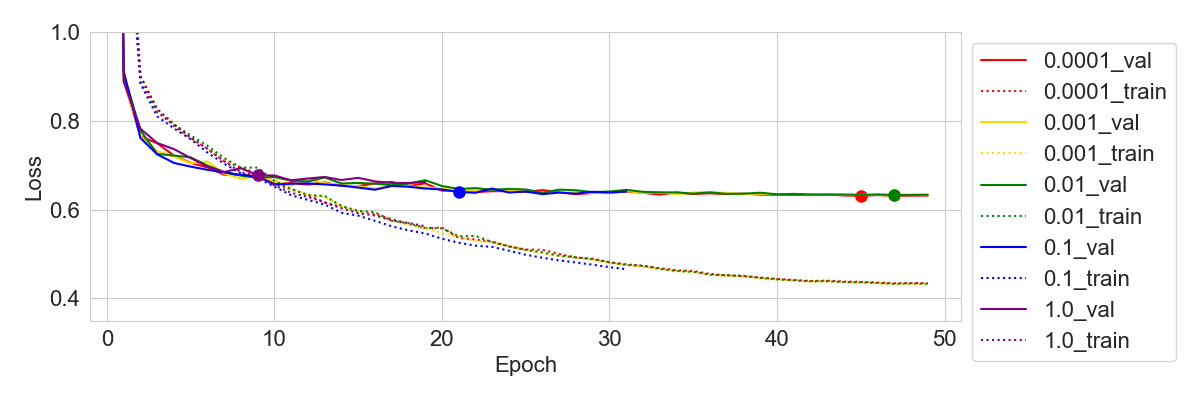
\includegraphics[height=55mm]{./figure/sec4/learning_curves/0/mel_loss.png}
        \caption{メルスペクトログラムのMAE Loss(式~\eqref{sec4:eq:loss}の$L_{mel}$)}
        \label{sec4:fig:learning_curve_baseline_val_mel_loss}
    \end{subfigure}
    \begin{subfigure}{\linewidth}
        \centering
        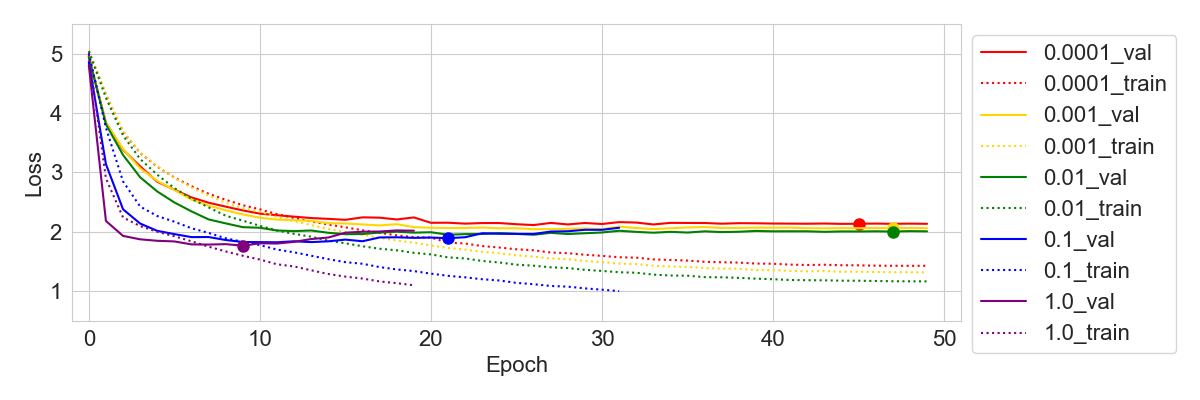
\includegraphics[height=55mm]{./figure/sec4/learning_curves/0/ssl_feature_cluster_loss.png}
        \caption{HuBERT離散特徴量のCross Entropy Loss(式~\eqref{sec4:eq:loss}の$L_{ssl^{d}}$)}
        \label{sec4:fig:learning_curve_baseline_val_ssl_feature_cluster_loss}
    \end{subfigure}
    \begin{subfigure}{\linewidth}
        \centering
        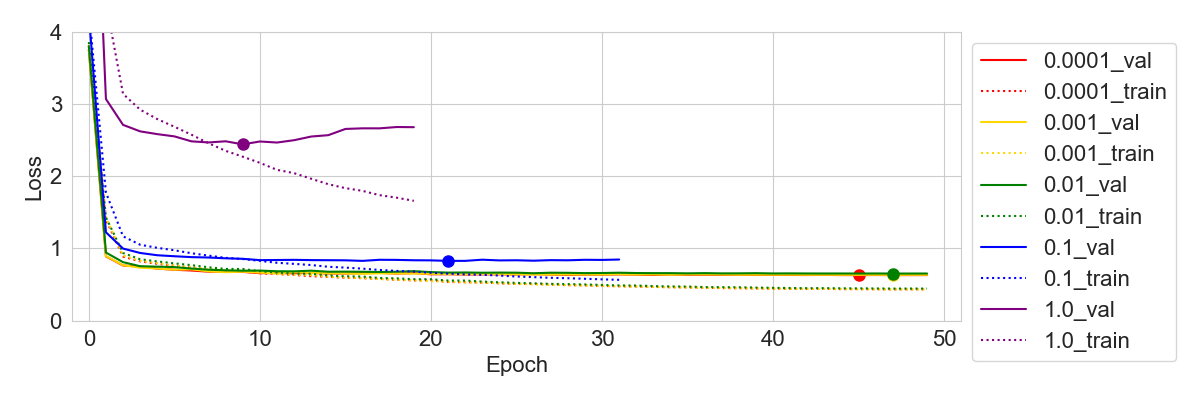
\includegraphics[height=55mm]{./figure/sec4/learning_curves/0/total_loss.png}
        \caption{損失の合計値(式~\eqref{sec4:eq:loss}の$L$)}
        \label{sec4:fig:learning_curve_baseline_val_total_loss}
    \end{subfigure}
    \caption{ベースラインにおける学習曲線}
    \label{sec4:fig:learning_curve_baseline_val_losses}
\end{figure}

\begin{figure}[bt]
    \centering
    \begin{subfigure}{\linewidth}
        \centering
        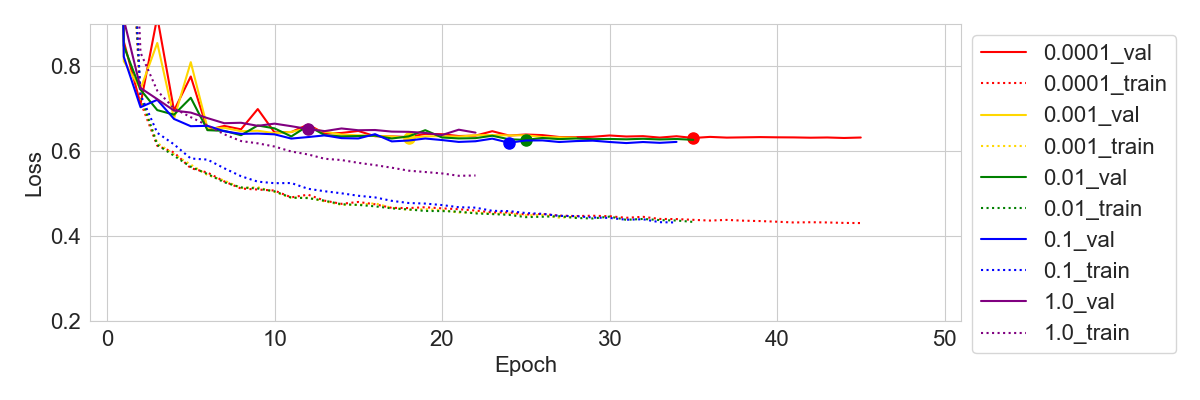
\includegraphics[height=55mm]{./figure/sec4/learning_curves/2/mel_loss.png}
        \caption{メルスペクトログラムのMAE Loss(式~\eqref{sec4:eq:loss}の$L_{mel}$)}
        \label{sec4:fig:learning_curve_method_2_val_mel_loss}
    \end{subfigure}
    \begin{subfigure}{\linewidth}
        \centering
        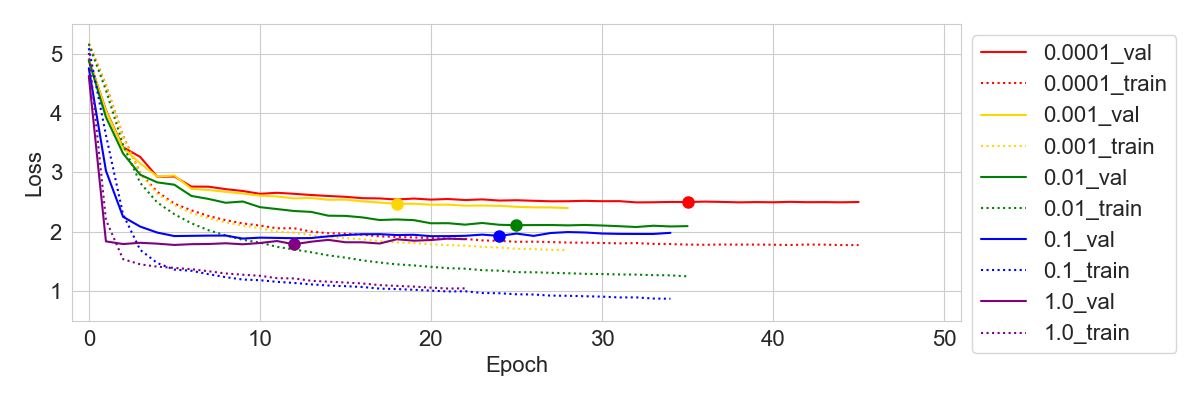
\includegraphics[height=55mm]{./figure/sec4/learning_curves/2/ssl_feature_cluster_loss.png}
        \caption{HuBERT離散特徴量のCross Entropy Loss(式~\eqref{sec4:eq:loss}の$L_{ssl^{d}}$)}
        \label{sec4:fig:learning_curve_method_2_val_ssl_feature_cluster_loss}
    \end{subfigure}
    \begin{subfigure}{\linewidth}
        \centering
        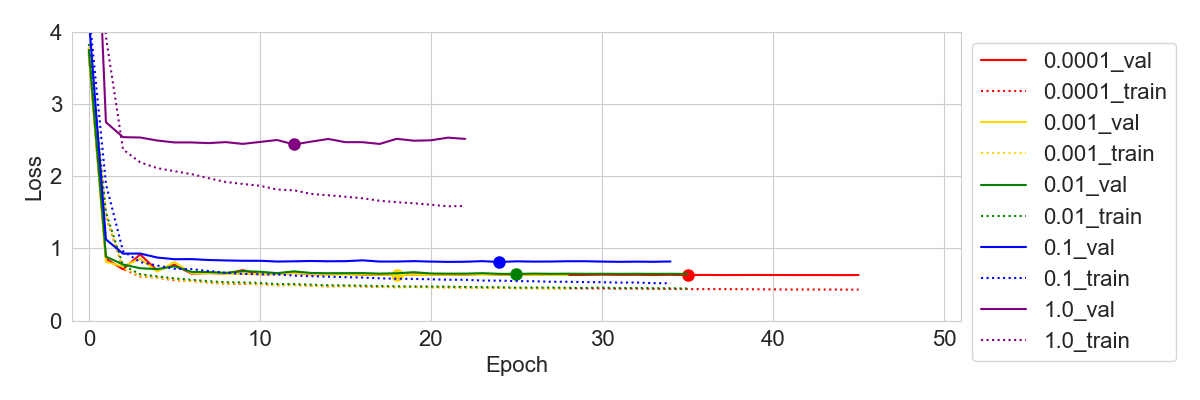
\includegraphics[height=55mm]{./figure/sec4/learning_curves/2/total_loss.png}
        \caption{損失の合計値(式~\eqref{sec4:eq:loss}の$L$)}
        \label{sec4:fig:learning_curve_method_2_val_total_loss}
    \end{subfigure}
    \caption{ネットワークB(Not-Pretrained)における学習曲線}
    \label{sec4:fig:learning_curve_method_2_val_losses}
\end{figure}

ベースラインでは、$\lambda_{ssl^{d}}$の値が0.001のときにWERが最も低く、0.01のときに話者類似度が最も高くなった。現状WERの高さが特に課題であり、話者類似度はほとんど同じであったため、今回は0.001が最適であると判断した。次に、図~\ref{sec4:fig:learning_curve_baseline_val_losses}にベースラインにおける学習曲線の結果を示す。横軸がエポック数、縦軸が損失の値を表す。損失の値は各エポックにおける平均値である。実線は検証データに対する損失、点線は学習データに対する損失を表しており、線の色は$\lambda_{ssl^{d}}$の違いを表す。また、丸いマーカーは表~\ref{sec4:tab:obj_method_comp}に示した最良エポック時における検証データに対する損失の値を表す。学習曲線より、$\lambda_{ssl^{d}}$の値を変化させることによって、特に$L_{ssl^{d}}$の傾向が変化していることがわかる。具体的には、$\lambda_{ssl^{d}}$の値を0.0001から1.0へと増加させるのに伴って、学習初期における損失の下がり方が急峻になっており、達する最小値自体が小さくなっていることがわかる。また、$\lambda_{ssl^{d}}$の値が0.1以上の場合、検証データに対する$L_{ssl^{d}}$は早いうちから増加傾向に転じている。これに伴い、今回は検証データに対する$L$の値を監視し、Early Stoppingの適用と最良エポックの決定を行なったため、$L_{mel}$が下がり切らない状態で学習が中断される結果となった。離散化して冗長性を排除したHuBERT離散特徴量と比較して、メルスペクトログラムが特に話者性を反映するために必要な特徴量だと考えられるため、$\lambda_{ssl^{d}}$が0.1以上の場合に見られた話者類似度の顕著な低下は、$L_{mel}$を下げきれなかったことが原因だと考えられる。

ネットワークAでは、提案手法の構成要素であるため、特に最適な手法の選択は行なっていない。ベースラインとの違いは$L_{ssl^{i}}$が損失に含まれることであるが、客観評価指標より、ベースラインと性能は概ね同等であることがわかる。学習曲線の傾向については、ベースラインと同様であったため省略する。

ネットワークB(Not-Pretrained)では、$\lambda_{ssl^{d}}$の値が0.1の時にWERが最も低く、0.0001の時に話者類似度が最も高くなった。ここではWERの低さを優先し、0.1が最適だと判断した。次に、図~\ref{sec4:fig:learning_curve_method_2_val_losses}にネットワークB(Not-Pretrained)における学習曲線の結果を示す。ベースラインと同様に、$\lambda_{ssl^{d}}$の値を0.0001から1.0へと増加させるのに伴って、学習初期における$L_{ssl^{d}}$の下がり方が急峻になっており、達する最小値自体が小さくなっていることがわかる。また、$\lambda_{ssl^{d}}$が1.0の場合に$L_{mel}$を下げきれなくなる傾向が見られ、ベースラインと同様にこのとき話者類似度の顕著な低下が確認された。加えて、ネットワークB(Not-Pretrained)では$\lambda_{ssl^{d}}$が0.1の場合における$L_{ssl^{d}}$の増加が緩やかであり、$L_{mel}$も十分下げられていることがわかる。さらに、$\lambda_{ssl^{d}}$が0.1の場合、$L_{mel}$の達する最小値自体が、$\lambda_{ssl^{d}}$が0.01以下の場合と比較して小さくなっていることがわかる。これはベースラインでは見られなかった新たな傾向であった。最適な$\lambda_{ssl^{d}}$の値は客観評価指標から0.1としたが、学習曲線の挙動より、この時他の値の場合と比較して$L_{mel}$と$L_{ssl^{d}}$の両方をバランスよく下げられていたと言える。

ネットワークC(Not-Pretrained)では、$\lambda_{ssl^{d}}$が0.1の場合が最適だと判断した。判断理由はネットワークB(Not-Pretrained)と同様である。学習曲線の傾向については、ネットワークB(Not-Pretrained)と同様であったため省略する。

ネットワークB(Pretrained)では、$\lambda_{ssl^{d}}$を0.1としたときにWERが最低となる一方で、0.01以上の場合と比較したときの話者類似度の低下が顕著であり、事前学習済み重みを読み込まなかったネットワークB(Not-Pretrained)とは異なる傾向であった。今回はWERが低いことを優先して、0.1が最適であると判断した。学習曲線の傾向については、ネットワークB(Not-Pretrained)と同様であったため省略する。学習曲線が同様であるにも関わらず結果の傾向が異なったことについては、重みの初期値が異なっていれば損失の値が同様だとしても異なる局所最適解に収束する可能性があるため、妥当だと判断した。

ネットワークC(Pretrained)では、$\lambda_{ssl^{d}}$の値が0.1の時にWERが最も低く、0.01の時に話者類似度が最も高くなった。ここでもWERが最低であることを優先して、0.1が最適だと判断した。学習曲線の傾向はネットワークB(Not-Pretrained)と同様であったため省略する。

次に、最適なチューニングをした場合における、手法ごとの客観評価指標の全テストデータに渡る平均値を表~\ref{sec4:tab:obj_method_comp}に示す。分析合成は、原音声から計算した特徴量を入力として、Multi-input Vocoderで逆変換した合成音声であり、本実験下において合成音声により達成され得る上限値を表す。ベースラインからネットワークC(Pretrained)については、表~\ref{sec4:tab:obj_weights}において太字としたもの、すなわち最適なチューニングだと判断されたものを選択している。また、ベースラインからネットワークC(Pretrained)の中で、最も優れた値を下線で示している。これより、提案手法であるネットワークB(Not-Pretrained)、ネットワークC(Not-Pretrained)、ネットワークC(Pretrained)の三つは、ベースラインに対してWERと話者類似度の両方を改善したことがわかる。一方、ネットワークB(Pretrained)はWERの改善を達成したが、話者類似度については悪化したことがわかる。ここで、HuBERTの事前学習済み重みを初期値とすることの効果について、ネットワークB(Not-Pretrained)とネットワークB(Pretrained)を比較すると、ネットワークB(Pretrained)の方がWERは1.1\%低いが、話者類似度も0.062低いことがわかる。実際に音声を聞いてみると、音声に不自然なノイズが含まれており、原音声に対する類似性が下がっていることが確認された。よって、HuBERTの事前学習済み重みを初期値としたHuBERT Transformer層の転移学習は、本タスクにおいて有効でないと考えられる。また、ネットワークCの導入効果について、ネットワークB(Not-Pretrained)とネットワークC(Not-Pretrained)を比較すると、ほとんど結果が変わらないことがわかる。一方、ネットワークB(Pretrained)とネットワークC(Pretrained)を比較すると、特に話者類似度についてネットワークC(Pretrained)はネットワークB(Pretrained)よりも0.071高いことがわかる。これより、ネットワークCの効果は、ベースとなるネットワークBの性能に依存して変化すると考えられる。

\begin{table*}[bt]
    \centering
    \caption{最適なチューニングをした場合における手法ごとの比較}
    \label{sec4:tab:obj_method_comp}
    \begin{center}
        \renewcommand{\arraystretch}{1.0} % 行の高さ調整
        \setlength{\tabcolsep}{8pt}      % 列の幅調整
        \scalebox{1.0}{
            \begin{tabular}{|c|l|rr|}
                \hline
                \multicolumn{1}{|c|}{手法} & \multicolumn{1}{c|}{$\lambda_{ssl^{d}}$} & \multicolumn{1}{c}{WER [\%]} & \multicolumn{1}{c|}{話者類似度} \\
                \hline
                ベースライン                   & 0.001                                    & 54.6                         & 0.836                      \\
                ネットワークB(Not-Pretrained)  & 0.1                                      & 45.3                         & 0.840                      \\
                ネットワークC(Not-Pretrained)  & 0.1                                      & 45.8                         & 0.848                      \\
                ネットワークB(Pretrained)      & 0.1                                      & \underline{44.2}             & 0.778                      \\
                ネットワークC(Pretrained)      & 0.1                                      & 45.5                         & \underline{0.849}          \\
                \hline
                分析合成                     & \multicolumn{1}{c|}{-}                   & 3.7                          & 0.956                      \\
                原音声                      & \multicolumn{1}{c|}{-}                   & 3.7                          & 1.000                      \\
                \hline
            \end{tabular}
        }
    \end{center}
\end{table*}

\subsubsection{客観評価2: 提案手法のさらなる検討}
\label{sec4:sec:obj_2}
本節では、\ref{sec4:sec:obj_1}節の客観評価によって得られた知見をもとに、さらなる提案手法の検討を行った結果を述べる。まず、\ref{sec4:sec:obj_1}節より、これまでに検討した提案手法の中で最も優れているのはネットワークB(Not-Pretrained)だと判断した。選択理由について、まずネットワークC(Not-Pretrained)とネットワークB(Not-Pretrained)はほとんど差がないため、ネットワークCの導入効果はほとんどないと判断しネットワークC(Not-Pretrained)を省いた。次に、ネットワークB(Pretrained)はネットワークB(Not-Pretrained)と比較してWERは1.2\%低いがその差は小さく、一方で話者類似度では顕著な低下が見られた。よって、ネットワークB(Pretrained)は本実験下においては効果的でないと判断した。最後に、ネットワークC(Pretrained)について、客観評価指標の値はネットワークB(Not-Pretrained)と同等であり、元となっているネットワークB(Pretrained)を省いたことも考慮して、ネットワークC(Pretrained)も省くこととした。

ネットワークB(Not-Pretrained)に対し、まずはHuBERT Transformer層への入力特徴量について検討した。\ref{sec4:sec:obj_1}節では事前学習済み重みを用いることの有効性を調べる目的があったため、入力は事前学習時に揃えてHuBERT中間特徴量としていた。しかし、選択したネットワークB(Not-Pretrained)は事前学習済み重みを利用しないため、HuBERT中間特徴量を入力とすることが意味をなしているか不明である。これに対し、今回はネットワークAからマルチタスク学習によって同時に予測される、メルスペクトログラムとHuBERT離散特徴量を入力とする場合を比較した。入力の際、メルスペクトログラムは連続したフレームをチャンネル方向に積んで、100Hz・80次元から50Hz・160次元に形状を変換した。HuBERT離散特徴量は、モデルから出力される予測確率分布をそのまま利用した。HiFi-GAN入力のように、一度トークンに変換してからベクトル表現を得るという手段も考えられたが、トークンに変換するためには予測確率を元にトークンをサンプリングする必要があり、これは微分不可能な操作であるため学習が不可能となる。そのため、ここでは予測確率分布をそのまま特徴量として利用することにした。パディング部のトークンを含むため、予測確率分布の次元は101次元である。これらを結合して$160 + 101 = 261$次元の特徴量とした上で、全結合層を通してHuBERT中間特徴量と同じ768次元までチャンネル数を上げ、HuBERT Transformer層への入力とした。これまでと同様に、五種類の$\lambda_{ssl^{d}}$でグリッドサーチを行った結果を表\ref{sec4:tab:obj_weights_networkb_input_comparison}に示す。新たに検討した手法はネットワークB(Not-Pretrained・Mel-Hub)とした。客観評価指標ごとに最も優れた値を下線で示しており、ネットワークB(Not-Pretrained・Mel-Hub)については最適だと判断した場合を太字で示している。これより、ネットワークB(Not-Pretrained・Mel-Hub)では、ネットワークB(Not-Pretrained)で見られたようなWERが下がる重みが確認されないことがわかる。最適だと判断した$\lambda_{ssl^{d}}$が0.001の場合においても、話者類似度はネットワークB(Not-Pretrained)よりも0.005とわずかに高いが、WERは10.1\%高い。これより、ネットワークB(Not-Pretrained・Mel-Hub)は、ネットワークB(Not-Pretrained)に劣ると判断した。この結果より、HuBERT中間特徴量はメルスペクトログラムとHuBERT離散特徴量の複合特徴量と比較して、ネットワークBの推定精度改善につながるより良い入力特徴量であったと考えられる。HuBERT中間特徴量は768次元であったのに対し、メルスペクトログラムとHuBERT離散特徴量の複合特徴量は261次元であるから、より高次元で冗長性が高い方が、ネットワークBによる特徴抽出の対象として優れていたのではないかと考える。

\begin{table*}[bt]
    \centering
    \caption{HuBERT Transformer層への入力特徴量を変化させた場合の比較}
    \label{sec4:tab:obj_weights_networkb_input_comparison}
    \begin{center}
        \renewcommand{\arraystretch}{1.0} % 行の高さ調整
        \setlength{\tabcolsep}{8pt}      % 列の幅調整
        \scalebox{0.98}{
            \begin{tabular}{|c|l|rr|}
                \hline
                \multicolumn{1}{|c|}{手法}                 & \multicolumn{1}{c|}{$\lambda_{ssl^{d}}$} & \multicolumn{1}{c}{WER [\%]} & \multicolumn{1}{c|}{話者類似度} \\
                \hline
                ネットワークB(Not-Pretrained・Mel-HuB)          & 0.0001                                   & 59.5                         & 0.840                      \\
                \textbf{ネットワークB(Not-Pretrained・Mel-HuB)} & \textbf{0.001}                           & \textbf{55.4}                & \underline{\textbf{0.845}} \\
                ネットワークB(Not-Pretrained・Mel-HuB)          & 0.01                                     & 56.2                         & 0.803                      \\
                ネットワークB(Not-Pretrained・Mel-HuB)          & 0.1                                      & 57.7                         & 0.795                      \\
                ネットワークB(Not-Pretrained・Mel-HuB)          & 1                                        & 58.1                         & 0.711                      \\
                \hline
                ネットワークB(Not-Pretrained)                  & 0.1                                      & \underline{45.3}             & 0.840                      \\
                \hline
            \end{tabular}
        }
    \end{center}
\end{table*}

次に、HuBERT中間特徴量をネットワークBに与えている、ネットワークAの学習方法を検討した。これまでの提案手法では、先行研究\cite{kim2023lip_multitask, choi2023intelligible}において報告されたマルチタスク学習の有効性を考慮し、ネットワークAにおいてHuBERT中間特徴量だけでなく、メルスペクトログラム、HuBERT離散特徴量を同時に予測するマルチタスク学習を採用していた。これに対し、ネットワークAにおいてHuBERT中間特徴量のみを推定するよう学習する場合を検討することで、マルチタスク学習の有効性を調べた。結果を表\ref{sec4:tab:obj_weights_networka_multitask}に示す。新たに検討した手法はネットワークB(Not-Pretrained・A-SingleTask)とした。客観評価指標ごとに最も優れた値を下線で示しており、ネットワークB(Not-Pretrained・A-SingleTask)については最適だと判断した場合を太字で示している。これより、ネットワークB(Not-Pretrained・A-SingleTask)で最適な場合を見ると、ネットワークB(Not-Pretrained)よりもWERが2.8\%低く、話者類似度は0.007高いことがわかる。従って、ネットワークAではネットワークBの入力に必要なHuBERT中間特徴量のみを推定する方が、メルスペクトログラムとHuBERT離散特徴量を同時に予測するマルチタスク学習を行うよりも、ネットワークBにより良い入力特徴量を与えられると考えられる。マルチタスク学習を行う場合、メルスペクトログラムやHuBERT離散特徴量が損失に加わるため、それらの損失を小さくするための勾配も考慮した重みの更新が行われるが、これがネットワークBに入力するHuBERT中間特徴量を推定する上では、悪影響を与えていると考えられる。

\begin{table*}[bt]
    \centering
    \caption{ネットワークAにおけるマルチタスク学習の有無による比較}
    \label{sec4:tab:obj_weights_networka_multitask}
    \begin{center}
        \renewcommand{\arraystretch}{1.0} % 行の高さ調整
        \setlength{\tabcolsep}{8pt}      % 列の幅調整
        \scalebox{0.96}{
            \begin{tabular}{|c|l|rr|}
                \hline
                \multicolumn{1}{|c|}{手法}                      & \multicolumn{1}{c|}{$\lambda_{ssl^{d}}$} & \multicolumn{1}{c}{WER [\%]} & \multicolumn{1}{c|}{話者類似度} \\
                \hline
                ネットワークB(Not-Pretrained・A-SingleTask)          & 0.0001                                   & 54.0                         & \underline{0.867}          \\
                ネットワークB(Not-Pretrained・A-SingleTask)          & 0.001                                    & 52.2                         & 0.865                      \\
                ネットワークB(Not-Pretrained・A-SingleTask)          & 0.01                                     & 51.8                         & 0.843                      \\
                \textbf{ネットワークB(Not-Pretrained・A-SingleTask)} & \textbf{0.1}                             & \underline{\textbf{42.5}}    & \textbf{0.847}             \\
                ネットワークB(Not-Pretrained・A-SingleTask)          & 1                                        & 43.0                         & 0.768                      \\
                \hline
                ネットワークB(Not-Pretrained)                       & 0.1                                      & 45.3                         & 0.840                      \\
                \hline
            \end{tabular}
        }
    \end{center}
\end{table*}

\subsubsection{主観評価}
主観評価実験は、本実験で検討した提案手法がベースラインに対する改善を達成したか否かを確認するために行った。\ref{sec4:sec:obj_1}節および\ref{sec4:sec:obj_2}節の検討結果より、本研究の提案手法の代表としては、ネットワークB(Not-Pretrained)と、ネットワークB(Not-Pretrained・SingleTask)を選択した。なぜなら、客観評価指標の結果から、最良だと考えられる提案手法はネットワークB(Not-Pretrained・SingleTask)であるが、ネットワークB(Not-Pretrained)もそれに次ぐ性能であり、ネットワークAにおけるマルチタスク学習の有無が主観評価において有意な差であるかも確かめたいと考えたからである。結果として、主観評価実験において比較する音声は以下の五種類である。
\begin{enumerate}
    \item ベースライン
    \item ネットワークB(Not-Pretrained)
    \item ネットワークB(Not-Pretrained・A-SingleTask)
    \item 分析合成
    \item 原音声
\end{enumerate}
\ref{sec4:sec:sbj_explanation}節で述べたように、主観評価では音声の明瞭性と類似性を五段階評価した。総被験者数は75人としたが、アプリの不具合によるエラーを理由に一名のデータを除き、それ以外の被験者についてはダミーサンプルの回答が正しかったためそのまま用いて、74名分のデータで統計処理を実施した。被験者の年齢層は21歳から62歳に渡った。年齢層の箱ひげ図を図\ref{sec4:fig:age}に示す。被験者の性別は男性32名、女性42名であった。また、実験に利用した音響機器はヘッドホンが18名、イヤホンが56名であった。
\begin{figure}[bt]
    \centering
    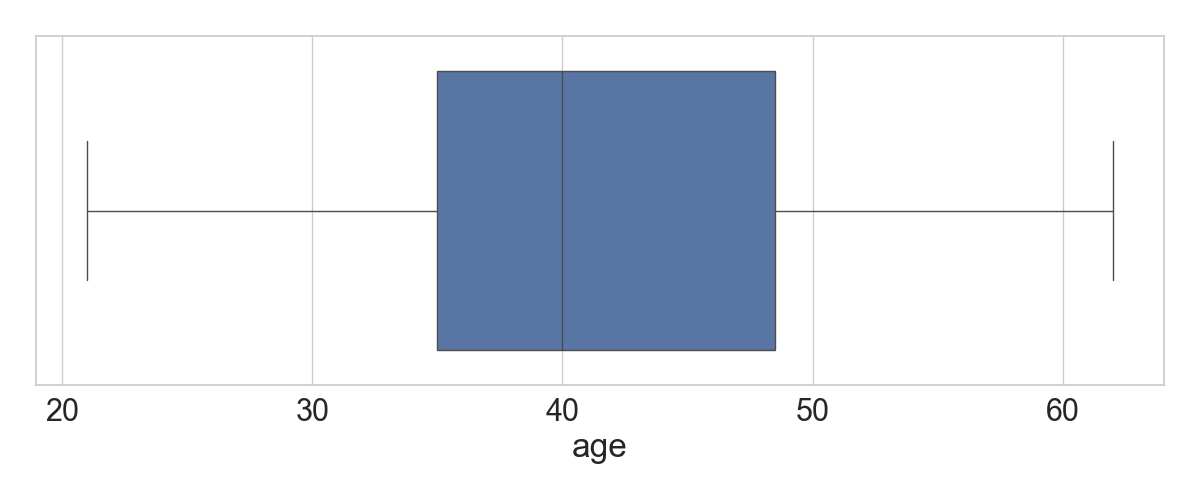
\includegraphics[height=50mm]{./figure/sec4/sbj/age.png}
    \caption{主観評価実験における被験者の年齢層}
    \label{sec4:fig:age}
\end{figure}

明瞭性と類似性の評価値について、手法ごとに平均値と95\%信頼区間を計算した結果を表\ref{sec4:tab:sbj_mean_ci}に示す。また、各手法の組み合わせについて、平均値の差の検定(片側検定)を行った結果を表\ref{sec4:tab:sbj_int_p}, \ref{sec4:tab:sbj_sim_p}に示す。表における$(i, j)$成分は、$i$行目の手法に対する評価値の母平均を$\mu_{i}$、$j$列目の手法に対する評価値の母平均を$\mu_{j}$とするとき、帰無仮説を$\mu_{i} = \mu_{j}$、対立仮説を$\mu_{i} > \mu_{j}$とした片側検定で計算されたp値に対し、Benjamini/Hochberg法による多重比較のための補正を行った結果である。ここで、表の文字列はそれぞれの以下の略称とする。
\begin{enumerate}
    \item GT: 原音声(Ground Truth)
    \item AbS: 分析合成(Analysis by Synthesis)
    \item B(N-P, A-S): ネットワークB(Not-Pretrained・A-SingleTask)
    \item B(N-P): ネットワークB(Not-Pretrained)
    \item Baseline: ベースライン
\end{enumerate}
また、本実験における有意水準は5\%とする。

まず、表\ref{sec4:tab:sbj_int_p}より、提案したネットワークB(Not-Pretrained)およびネットワークB(Not-Pretrained・A-SingleTask)は、ベースラインに対して明瞭性の評価値が有意に高いことがわかる。これより、二つの提案手法はどちらもベースラインより話者の想定した発話内容を正確に反映した合成音声を実現できたと考えられる。一方、提案手法二つの間には有意差がないことも分かる。これより、ネットワークAの学習方法の違いは明瞭性に有意な差をもたらさなかったと言える。次に、表\ref{sec4:tab:sbj_sim_p}より、提案したネットワークB(Not-Pretrained)およびネットワークB(Not-Pretrained・A-SingleTask)は、ベースラインに対して類似性の評価値が有意に高いことがわかる。これより、二つの提案手法はどちらもベースラインより原音声に似た合成音声を実現できたと考えられる。また、ここでは提案手法二つの間にも有意差があることが分かる。これより、ネットワークAの学習方法の違いは明瞭性に有意な差をもたらさなかったが、類似性には有意な差をもたらしたと言える。

以上のことから、ネットワークB(Not-Pretrained・A-SingleTask)が明瞭性・類似性の両面において、最も優れた合成音声を実現したと考えられる。一方、ネットワークB(Not-Pretrained・A-SingleTask)と、合成音声の性能上限を表す分析合成の間には未だ大きな差があり、特に自然音声に迫る合成音の実現は達成されていない。従って、本実験におけるベースラインからの改善は達成したものの、今後もさらなるネットワークの改善が必要だと考えられる。

\begin{table*}[bt]
    \centering
    \caption{主観評価実験の結果より計算した標本平均と95\%信頼区間}
    \label{sec4:tab:sbj_mean_ci}
    \begin{center}
        \renewcommand{\arraystretch}{1.0} % 行の高さ調整
        \setlength{\tabcolsep}{8pt}      % 列の幅調整
        \scalebox{0.95}{
            \begin{tabular}{|c|l|rr|}
                \hline
                \multicolumn{1}{|c|}{手法}             & \multicolumn{1}{c|}{$\lambda_{ssl^{d}}$} & \multicolumn{1}{c}{明瞭性} & \multicolumn{1}{c|}{類似性} \\
                \hline
                ベースライン                               & 0.001                                    & $2.371 \pm 0.072$       & $2.933 \pm 0.080$        \\
                ネットワークB(Not-Pretrained)              & 0.1                                      & $2.753 \pm 0.075$       & $3.052 \pm 0.085$        \\
                ネットワークB(Not-Pretrained・A-SingleTask) & 0.1                                      & $2.818 \pm 0.079$       & $3.182 \pm 0.082$        \\
                \hline
                分析合成                                 & \multicolumn{1}{c|}{-}                   & $4.749 \pm 0.040$       & $4.316 \pm 0.071$        \\
                原音声                                  & \multicolumn{1}{c|}{-}                   & $4.866 \pm 0.032$       & $4.705 \pm 0.052$        \\
                \hline
            \end{tabular}
        }
    \end{center}
\end{table*}

\begin{table*}[bt]
    \centering
    \caption{主観評価実験の結果より計算した平均値の差の検定におけるp値(明瞭性)}
    \label{sec4:tab:sbj_int_p}
    \begin{center}
        \renewcommand{\arraystretch}{1.0} % 行の高さ調整
        \setlength{\tabcolsep}{8pt}      % 列の幅調整
        \scalebox{0.95}{
            \begin{tabular}{|c|rrrr|}
                \hline
                \multicolumn{1}{|c|}{} & \multicolumn{1}{c}{AbS} & \multicolumn{1}{c}{B(N-P, A-S)} & \multicolumn{1}{c}{B(N-P)} & \multicolumn{1}{c|}{Baseline} \\
                \hline
                GT                     & $5.25 \times 10^{-6}$   & $2.14 \times 10^{-259}$         & $2.82 \times 10^{-285}$    & $0$                           \\
                AbS                    & \multicolumn{1}{c}{-}   & $2.23 \times 10^{-240}$         & $4.56 \times 10^{-266}$    & 0                             \\
                B(N-P, A-S)            & \multicolumn{1}{c}{-}   & \multicolumn{1}{c}{-}           & $1.23 \times 10^{-1}$      & $3.61 \times 10^{-16}$        \\
                B(N-P)                 & \multicolumn{1}{c}{-}   & \multicolumn{1}{c}{-}           & \multicolumn{1}{c}{-}      & $5.77 \times 10^{-13}$        \\
                \hline
            \end{tabular}
        }
    \end{center}
\end{table*}

\begin{table*}[bt]
    \centering
    \caption{主観評価実験の結果より計算した平均値の差の検定におけるp値(類似性)}
    \label{sec4:tab:sbj_sim_p}
    \begin{center}
        \renewcommand{\arraystretch}{1.0} % 行の高さ調整
        \setlength{\tabcolsep}{8pt}      % 列の幅調整
        \scalebox{0.95}{
            \begin{tabular}{|c|rrrr|}
                \hline
                \multicolumn{1}{|c|}{} & \multicolumn{1}{c}{AbS} & \multicolumn{1}{c}{B(N-P, A-S)} & \multicolumn{1}{c}{B(N-P)} & \multicolumn{1}{c|}{Baseline} \\
                \hline
                GT                     & $1.07 \times 10^{-17}$  & $1.93 \times 10^{-156}$         & $1.17 \times 10^{-169}$    & $1.01 \times 10^{-200}$       \\
                AbS                    & \multicolumn{1}{c}{-}   & $1.31 \times 10^{-82}$          & $5.25 \times 10^{-96}$     & $3.53 \times 10^{-118}$       \\
                B(N-P, A-S)            & \multicolumn{1}{c}{-}   & \multicolumn{1}{c}{-}           & $1.70 \times 10^{-2}$      & $1.34 \times 10^{-5}$         \\
                B(N-P)                 & \multicolumn{1}{c}{-}   & \multicolumn{1}{c}{-}           & \multicolumn{1}{c}{-}      & $2.29 \times 10^{-2}$         \\
                \hline
            \end{tabular}
        }
    \end{center}
\end{table*}

\clearpage

\subsection{まとめ}

\clearpage

\section{結論}

\clearpage

\section*{謝辞}
\addcontentsline{toc}{section}{謝辞}

\clearpage

\bibliographystyle{junsrt}
\addcontentsline{toc}{section}{参考文献}
\bibliography{library}

\end{document}